%! Author = samuel
%! Date = 21/9/22

% Preamble
\documentclass[12pt]{report}

% Packages
% Spanish-specific commands
\usepackage[spanish]{babel}
% Set the font (output) encodings
\usepackage[T1]{fontenc}
% Set the input encoding
\usepackage[utf8]{inputenc}
\usepackage{extramarks} % Todo: check if this can be removed or not
\usepackage[hidelinks]{hyperref} % Automatic links in TOC and hides red border
\usepackage{amsmath}
\usepackage{amssymb}
\usepackage{csquotes}
\usepackage{caption}
\usepackage{geometry}
\usepackage{tabularx}
\usepackage{graphicx}
\usepackage{fancyhdr}
\usepackage{lastpage}
\usepackage{setspace}
\usepackage{color}
\usepackage{pagecolor}
\usepackage{lib/tikz-uml}
\usepackage[explicit,compact]{titlesec}
\usepackage[cache=false]{minted}
\usepackage{pdfpages}

\usemintedstyle{manni}

\usepackage[backend=biber,sorting=none]{biblatex}
\addbibresource{bibliography.bib}

% Todo: Delete when making the final document
%\pagecolor{white!55!black}

% Set the margins to the pages
\geometry{
	a4paper,
	top=3cm,
	left=3cm,
	bottom=2.5cm,
	right=2.5cm
}
\title{Trabajo Final de Grado}
\author{C.D. Samuel}
\date{June 2023}

\pagestyle{fancy}
\renewcommand{\sectionmark}[1]{\markright{\textsl{\thesection.\ #1}}}
%\fancyhead{} % Clear all header fields
%\fancyhead[R]{Página \thepage\ de~\pageref{LastPage}} % Ignore warning
%\fancyhead[L]{\rightmark}
%\fancyfoot{} % Clear all footer fields
%\fancyfoot[R]{Samuel Castrillo Domínguez}
%\fancyfoot[L]{
%	\raisebox{-0.4\height}{
\includegraphics[scale=0.36]{imageULE}}
%}

% Horizontal line at top and bottom of page
\renewcommand{\headrulewidth}{0.5pt}
\renewcommand{\footrulewidth}{0.2pt}

%\fancypagestyle{plain}{ % Index and chapter pages
%	\fancyhf{} % Clear header and footer
%	\fancyhead[R]{\thepage}
%	\renewcommand{\footrulewidth}{0pt}
%}

\newcommand{\chapterFont}[1]{{\bfseries{\fontsize{28pt}{0pt}\selectfont{#1}}}}
\newcommand{\sectionFont}[1]{{\bfseries{\uppercase{\fontsize{14pt}{0pt}\selectfont{#1}}}}}

% See docs: http://tug.ctan.org/tex-archive/macros/latex/contrib/titlesec/titlesec.pdf
\titleformat{\chapter}[hang]{\bfseries}{\chapterFont{\thechapter.}}{15pt}{\chapterFont{#1}}
\titleformat{\section}[hang]{\bfseries}{\sectionFont{\thesection.}}{15pt}{\sectionFont{#1}}
\titleformat{\subsection}[hang]{\bfseries}{\sectionFont{\thesubsection.}}{15pt}{\sectionFont{#1}}

% Espaciado entre títulos y texto (ver https://tex.stackexchange.com/questions/53338/reducing-spacing-after-headings)
\titlespacing*{\chapter}{0pt}{-5pt}{12pt} % Remove space before chapter title
\titlespacing*{\section}{0pt}{18pt}{12pt}
\titlespacing*{\subsection}{0pt}{18pt}{12pt}
\titlespacing*{\subsubsection}{0pt}{18pt}{12pt}

\newcommand{\chaptr}[2]{\chapter{#1}\label{ch:#2}}
\newcommand{\sect}[2]{\section{#1}\label{sec:#2}}
\newcommand{\subsect}[2]{\subsection{#1}\label{subsec:#2}}
\newcommand{\subsubsect}[2]{\subsubsection{#1}\label{subsubsec:#2}}

\newcommand{\monoFont}[1]{\texttt{#1}}
\newcommand{\boldFont}[1]{\textbf{#1}}
\newcommand{\boldmonoFont}[1]{\textbf{\texttt{#1}}}

\captionsetup{width=0.8\textwidth}
\usepackage{newfloat}

% placement = H means that the float environment will be placed where the \begin{} command is, estrictly.

\DeclareFloatingEnvironment[
	fileext = cod,
	listname = {Índice de bloques de código},
	name = Código,
	placement = H,
]{codeBlock}

\DeclareFloatingEnvironment[
	fileext = dia,
	listname = {Índice de diagramas UML},
	name = Diagrama UML,
	placement = H % See docs -> https://www.overleaf.com/learn/latex/Positioning_images_and_tables#The_figure_environment
]{umlDiagram}


\newcommand{\str}[1]{``{#1}''}
\newcommand{\quoted}[1]{\textquoteleft#1\textquoteright}

\renewcommand{\labelenumii}{\arabic{enumi}.\arabic{enumii}.}
\renewcommand{\labelenumiii}{\arabic{enumi}.\arabic{enumii}.\arabic{enumiii}.}
\renewcommand{\labelenumiv}{\arabic{enumi}.\arabic{enumii}.\arabic{enumiii}.\arabic{enumiv}.}

\newcommand{\emoji}[1]{\raisebox{-0.2em}{\includegraphics[width=1em]{lib/emojis/#1}}}


\usepackage[automake]{glossaries}
\usepackage{eurosym}
\usepackage{booktabs}

\makeglossaries
\loadglsentries{glosario}
\glsaddall

\captionsetup{width=0.8\textwidth, justification=centerlast}

% Change font and line spacing of UML diagrams
\tikzumlset{font=\fontsize{10pt}{8pt}\selectfont\ttfamily}

% Document
\begin{document}
	\thispagestyle{empty}
\graphicspath{{./res/images/}}

% Table for the cover
\begin{table}[ht]
	\centering

	% Images at the top of the cover
	\hfill
	\\[-10ex]
	
\includegraphics{imageULE}
	\hfill
	
\includegraphics{imageInformatica}
	\\[10ex]

	\label{tab:coverTopCenter}
	\begin{tabular}{p{1\linewidth}}
		\centering
		\LARGE\textbf{Escuela de Ingenierías}
		\\[1.5ex]

		\LARGE\textbf{Industrial, Informática y} \\
		\LARGE\textbf{Aeroespacial}
		\\[2.3ex]

		\LARGE\textbf{GRADO EN INGENIERÍA INFORMÁTICA}
		\\[5ex]

		\LARGE{Trabajo de Fin de Grado}
		\\[5ex]

		\LARGE{\uppercase{Aplicación web de chat para comunicación en tiempo real entre estudiantes y docentes. RS Chat}}
		\\[5ex]

		\LARGE{\uppercase{Real time chat web application for students and teachers communication. RS Chat}}
		\\[8ex]

		\hfill\large{Autor: Samuel Castrillo Domínguez}
		\\[3pt]
		\hfill\large{Tutor: Eva María Cuervo Fernández}
		\\[5ex]

		\huge{Junio, 2023}
	\end{tabular}
\end{table}

	\clearpage
	\thispagestyle{empty}

\begin{table}[ht]
	\centering
	\label{tab:info}
	\begin{tabularx}{\textwidth}{|X|X|}
		\hline

		\begin{center}
			\LARGE\textbf{UNIVERSIDAD DE LEÓN} \\[4pt]
			\LARGE\textbf{Escuela de Ingenierías Industrial, Informática y} \\
			\LARGE\textbf{Aeroespacial} \\[16pt]
			\LARGE\textbf{GRADO EN INGENIERÍA INFORMÁTICA} \\[4pt]
			\LARGE\textbf{Trabajo de Fin de Grado} \\[35pt]
		\end{center}
		\\

		\hline

		\\[-6.6ex]
		\begin{flushleft}
			\textbf{ALUMNO:} Samuel Castrillo Domínguez
		\end{flushleft}
		\\[-3ex]

		\hline

		\\[-6.6ex]
		\begin{flushleft}
			\textbf{TUTOR:} Eva María Cuervo Fernández
		\end{flushleft}
		\\[-3ex]

		\hline

		\\[-7ex]
		\begin{flushleft}
			\textbf{TÍTULO:} RS Chat: Aplicación web de chat para comunicación en tiempo real entre estudiantes y docentes.
		\end{flushleft}
		\\[-3ex]

		\hline

		\\[-6.6ex]
		\begin{flushleft}
			\textbf{TITLE:} RS Chat: Real time chat web application for students and teachers communication.
		\end{flushleft}
		\\[-3ex]

		\hline

		\\[-6.6ex]
		\begin{flushleft}
			\textbf{CONVOCATORIA:} Junio, 2023
		\end{flushleft}
		\\[-3ex]

		\hline

		\\[-6.6ex]
		\begin{flushleft}
			\textbf{RESUMEN:} \\
			{El resumen reflejará las ideas principales de cada una de las partes del
			trabajo, pudiendo incluir un avance de los resultados obtenidos. Constará de
			un único párrafo y se recomienda una longitud no superior a 300 palabras. En
			cualquier caso, no deberá superar una página de longitud.}
		\end{flushleft}
		\\[-1.5ex]

		\hline

		\\[-6.6ex]
		\begin{flushleft}
			\textbf{ABSTRACT:} \\
			{Abstract will reflect the main ideas of each part of the work, including
			an advance of the results obtained. It will consist of a single paragraph and
			it is recommended a length not superior to 300 words. In any case, it should
			not exceed a page of length.}
		\end{flushleft}
		\\[-1.5ex]

		\hline

		\\[-6.8ex]
		\begin{flushleft}
			\textbf{Palabras clave:} Lorem, ipsum, dolor, sit, amet.
		\end{flushleft}
		\\[-3ex]

		\hline

		\begin{tabular}{p{0.45\textwidth}|p{0.5\textwidth}}
			\textbf{Firma del alumno:}
			&
			\textbf{VºBº Tutor/es:} \\

			% Leave some blank space
			{} & {} \\[10ex]
		\end{tabular}
		\\

		\hline
	\end{tabularx}
\end{table}


	\clearpage

	\renewcommand{\contentsname}{Índice de contenidos}
	\pagenumbering{roman}
	\tableofcontents

	\cleardoublepage
	\listoffigures
	\addcontentsline{toc}{chapter}{\listfigurename}

	\cleardoublepage
	\renewcommand{\listtablename}{Índice de cuadros y tablas}
	\listoftables
	\addcontentsline{toc}{chapter}{\listtablename}

	\cleardoublepage
	\listofcodeBlocks
	\addcontentsline{toc}{chapter}{\listcodeBlockname}

	\cleardoublepage
	\listofumlDiagrams
	\addcontentsline{toc}{chapter}{\listumlDiagramname}

	\clearpage
	\printglossary[nonumberlist]
	\addcontentsline{toc}{chapter}{Glosario}

	\clearpage
	\pagenumbering{arabic} % Reset to normal numbers from here

	\begin{spacing}{1.5}
		\chaptr{Introducción}{introducción}
\sect{Patrones de diseño utilizados}{design-patterns}

Definición: \textit{Se trata de una solución que se puede aplicar a diferentes contextos y que se
puede reutilizar en diferentes proyectos.} \\

En este proyecto se han utilizado varios patrones de diseño, para permitir una mejor escalabilidad, mantenibilidad y
reutilización del código.\ A continuación se detallan los patrones utilizados y su justificación.

\subsect{Builder}{builder}


\subsect{Singleton}{singleton}
Este patrón se utiliza para garantizar que una clase tenga una única instancia y proporciona un punto de acceso
global a ella~\cite{sarcar2018java}.\ En el contexto de esta aplicación, se utiliza en ciertas
clases de utilidad y en las clases que asocian rutas a un método HTTP (por ejemplo \mono{/login} con el método POST).
Estas últimas son clases internas de \mono{Routes.java} y los nombres dependen del método HTTP que se debe utilizar para
realizar una petición a una ruta específica.

\begin{table}[ht]
	\centering
	\label{tab:routes}
	\begin{tabular}{|c|c|}
		\hline
		Método HTTP & Clase de la ruta   \\
		\hline
		GET           & \mono{GetRoute}    \\
		POST          & \mono{PostRoute}   \\
		PUT           & \mono{PutRoute}    \\
		DELETE        & \mono{DeleteRoute} \\
		\hline
	\end{tabular}
	\caption{Relación entre ruta y clase HTTP}
\end{table}

%\begin{lstlisting}[label={lst:lstlisting}]
%public class Routes {
%	private Routes() {
%	}
%	...
%	public static class GetRoute {
%	    public static final GetRoute INSTANCE = new GetRoute();
%		private GetRoute() {
%		}
%		public static final String USERS_URL = V_1 + "/users";
%		...
%	}
%	...
%}
%\end{lstlisting}

Código
\begin{minted}{c}
int main() {
	printf("hello, world");
	return 0;
}
\end{minted}

\subsect{Strategy}{strategy}


\sect{Procesamiento de los mensajes}{procesamiento-mensajes}

Como hemos visto en la sección anterior, los mensajes que se reciben en el servidor pueden ser de diferentes tipos,
cambiando la forma en que se procesan.\ A continuación se muestra una lista con las acciones que se realizan para
cada tipo de mensaje que se trata:

\begin{itemize}
	\item \boldFont{Text, Image, Video y Audio}: se envían al resto de usuarios del chat en el mismo formato en que llegaron al
	servidor.\ Estos cuatro tipos de mensaje contienen texto exclusivamente, siendo un mensaje o el enlace a un
	archivo almacenado en el bucket de S3.
	\item \boldFont{ActiveUsers}: se envía solo al cliente que lo ha solicitado, y contiene una lista con los usuarios que están
	conectados en ese momento al chat, ordenados alfabéticamente.
	\item \boldFont{GetHistory}: se envía al usuario que lo solicita, y contiene una lista con los últimos 65 mensajes que se han
	enviado al chat.\ Se realiza una lectura del fichero de texto que contiene el historial de mensajes (almacenado
	en disco) y un filtrado de los mensajes de actividad (los 2 siguientes) del solicitante, ya que no son relevantes.
	\item \boldFont{UserJoined y UserLeft}: se notifica a las personas conectadas el nombre del usuario que se ha unido o ha
	salido del chat, % todo (implementar): y se envía a todos los usuarios la lista de usuarios conectados actualizada.
	\item \boldFont{Ping}: se envía un mensaje con un breve texto.\ Se utiliza exclusivamente para mantener la conexión WebSocket
	abierta.
\end{itemize}

\sect{Ciclo de vida de la conexión de usuarios}{ciclo-de-vida-conexión-usuario}

Cuando un usuario accede a un chat de la aplicación, se inicia una conexión entre el cliente y el servidor a través
del protocolo de comunicación bidireccional \boldFont{WebSocket}~\cite{RFCWebSocket}.\ Esta conexión se mantiene
abierta mientras el
usuario esté en el chat, y se cierra cuando el usuario lo abandona.\ La secuencia de eventos que ocurren durante
la conexión de un usuario al chat es la siguiente:

\subsect{Frontend}{frontend}

\begin{enumerate}
	\item Se realiza una solicitud de conexión WebSocket al servidor.
	\item Se realiza una petición HTTP para comprobar que el usuario puede acceder al chat.\ Esto se realiza para
	que, en caso de que el usuario introduzca la URL de un chat al que no tiene acceso de forma manual, se le redirija
	a la página de inicio de la aplicación.
	\item Si se confirma que el usuario \boldFont{puede acceder} al chat:
	\begin{enumerate}
		\item Se establece la conexión WebSocket.
		\item Se envía un mensaje de tipo \monoFont{USER\_JOINED} al servidor.
		\item Se consultan los últimos mensajes del historial de mensajes del chat con el mensaje de tipo
		\monoFont{GET\_HISTORY\_MESSAGE}.
		\item Se realiza una petición de la lista de usuarios activos con un mensaje de tipo
		\monoFont{ACTIVE\_USERS\_MESSAGE}.
		\item Se configura un temporizador para mandar un mensaje de tipo \monoFont{PING\_MESSAGE} cada 30 segundos.
		Esto se realiza para que el servidor no cierre la conexión por inactividad.
	\end{enumerate}
	\item Si el usuario \boldFont{no puede acceder} al chat:
	\begin{enumerate}
		\item Se cierra la conexión WebSocket, en caso de llegarse a abrir.
		\item Se redirige al usuario a la página principal.
	\end{enumerate}
\end{enumerate}
\label{itm:frontend-connection-life-cycle}

\subsect{Backend}{backend}

Cuando comienza la ejecución del programa, se indica a Spring Boot que el manejador de mensajes a través de WebSocket
del servidor es una instancia de la clase \monoFont{WebSocketHandler}, en la ruta
\quoted{/ws/rschat}.\ Al instanciar esta clase, se crea un objeto \boldFont{chatMap} de tipo
\monoFont{WebSocketChatMap}, que contiene el atributo
\monoFont{chats} (ver Diagrama UML~\ref{diagram-WebSocketChatMapClass}).\ Es una tabla de dispersión que contiene los
chats activos en la aplicación.\ Cada entrada asocia a una cadena de texto (identificador del chat) la instancia de
un objeto de tipo \monoFont{Chat}.\ El proceso de \boldFont{conexión} al servidor sigue el siguiente flujo de eventos:

\begin{enumerate}
	\item Se establece la conexión WebSocket con el usuario.\ Esto ocurre de forma transparente al programador debido a
	que la implementación se realiza en el framework de Spring Boot.
	\item Se recibe el mensaje \monoFont{USER\_JOINED} del cliente y se crea un objeto de tipo \monoFont{WSClient}
	(formado por la instancia de \monoFont{WebSocketSession} y el \monoFont{WSClientID} del usuario).\ Este nuevo
	objeto se añade a la lista de usuarios conectados al chat.
	\begin{enumerate}
		\item Si el usuario es el primero que se ha conectado al chat, se crea uno nuevo, guardándose en la lista de
		chats.
		\item Si no, se añade al chat correspondiente de la lista de chats.
	\end{enumerate}
	\item Se recibe el mensaje \monoFont{GET\_HISTORY\_MESSAGE} del cliente y se envían como respuesta los últimos 65
	mensajes del historial de mensajes del chat.
	\item Se recibe el mensaje \monoFont{ACTIVE\_USERS\_MESSAGE} del cliente y se devuelve la lista con los usuarios
	activos en el chat.
\end{enumerate}
\label{itm:backend-connection-life-cycle}
Y el proceso de \boldFont{desconexión} se realiza como sigue:

\begin{enumerate}
	\item Se recibe el mensaje \monoFont{USER\_LEFT} del cliente.
	\item Se informa al resto de los usuarios del chat de la desconexión del usuario.
	\item Al eliminar un usuario del chat se pueden dar 2 casos:
	\begin{enumerate}
		\item Si el usuario es el último que se ha desconectado del chat, se elimina el chat de la tabla de dispersión
		\monoFont{chats}.\ Cuando esto ocurre, el historial de mensajes del chat que se haya registrado desde que se
		inició, se envía al almacenamiento en la nube.
		\item Si no, se elimina el usuario de la lista de usuarios del chat.
	\end{enumerate}
	\item Se cierra la conexión WebSocket con el usuario, de forma transparente al programador (al igual que la
	conexión).
\end{enumerate}

\begin{umlDiagram}
	\centering

	\begin{tikzpicture}
		\umlclass{WebSocketChatMap}{
			-- Map~<String, Chat>~ chats
		}{
			-- createChat(String): void \\
			-- chatExists(String): boolean \\
			-- getClientsOf(String): List~<WSClient> \\
			-- saveMessage(String, String): void \\
			+ getClient(WSClientID): WSClient \\
			+ addClientToChat(WSClient): void \\
			+ removeClientFromChat(WSClientID): void \\
			+ broadcastToSingleChat(String, String): void \\
			+ broadcastToSingleChatAndExcludeClient(WSClientID, String): void \\
			+ totalBroadcast(String): void \\
			+ getUsernamesOfChat(String): List~<String> \\
			-- saveAllToS3(): void \\
			-- deleteNullUsers(): void
		}{}
		\umlnote[y=-5.5,width=8.5cm]{WebSocketChatMap}{
			Los dos últimos métodos se ejecutan de manera periódica cada 10 y 3 minutos respectivamente.
		}{}
	\end{tikzpicture}

	\caption{Clase \monoFont{Chat} para almacenar los usuarios activos}
	\label{diagram-WebSocketChatMapClass}
\end{umlDiagram}

% Loki docker plugin causes all the containers to be unable to restart or kill. The alternative is to use the
% json-file driver with custom options. The json-file driver is the default driver for Docker.
% https://stackoverflow.com/questions/38567355/docker-compose-global-level-logging
% https://howchoo.com/devops/how-to-add-a-health-check-to-your-docker-container

\sect{Docker}{docker}
Docker es una plataforma software que permite el desarrollo, prueba y ejecución de aplicaciones de forma rápida y
cómoda, separando la aplicación de la infraestructura permitiendo ejecutar múltiples aplicaciones en un mismo servidor
(ver imagen~\ref{fig:docker-container-infrastructure}).\ Esto se realiza empaquetando la
aplicación, sus dependencias y otras herramientas necesarias para su ejecución en lo que se denominan
\boldFont{contenedores}, que son instancias ejecutables de una imagen de Docker.\ Las imágenes son ficheros de solo
lectura que contienen las instrucciones necesarias para crear un contenedor y normalmente se basan en otras imágenes
añadiendo o modificando configuraciones~\cite{docker-docs}.

\begin{figure}[ht]
	\centering
	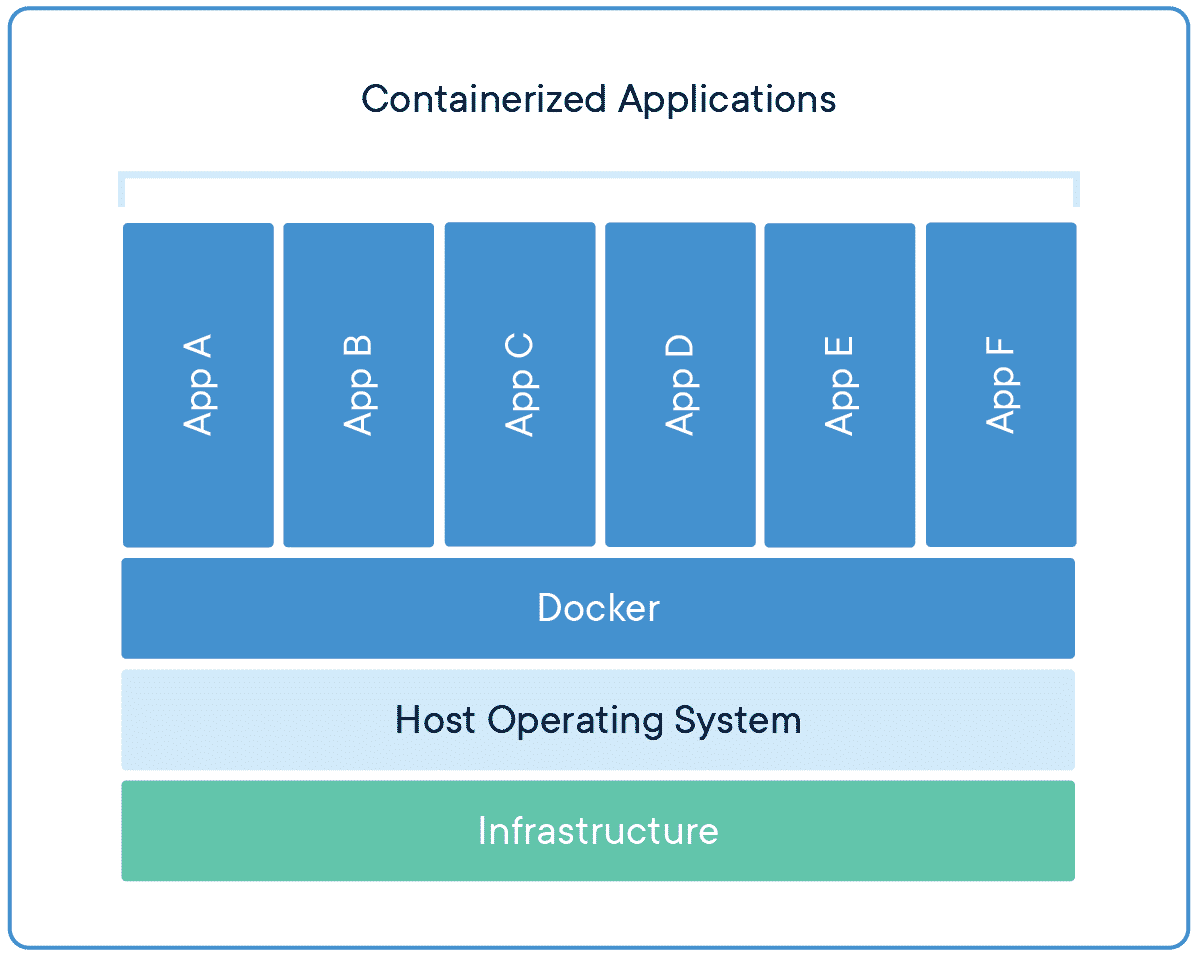
\includegraphics[width=0.8\textwidth]{res/images/container-what-is-container}
	\caption{Infrastructura docker. Fuente: \url{https://www.docker.com/resources/what-container}}
	\label{fig:docker-container-infrastructure}
\end{figure}

En el desarrollo de la aplicación se ha utilizado Docker para la creación de una imagen que contenga todo el código de
la aplicación así como las variables de entorno necesarias para su correcto funcionamiento.\ Se ha
utilizado la herramienta \monoFont{docker-compose}, que permite definir y ejecutar contenedores Docker de manera
sencilla.\ Para la configuración de los contenedores, se dispone del fichero \monoFont{docker-compose.yml} que se
encuentra en la raíz del proyecto y define los servicios que se ejecutarán en los contenedores, así como
las dependencias entre ellos.

Debido a que cada vez que se elimina un contenedor (al reiniciar el sistema o al generar de nuevo la imagen de la
aplicación para incluir cambios del código) se pierden los datos, la persistencia de los mismos y de sus
configuraciones es necesaria.\ Para lograr esto, se usan \boldFont{volúmenes}, que son directorios creados y
gestionados por Docker que se almacenan en el sistema de archivos del host, y que se montan en los contenedores cuando
se inicializan~\cite{docker-volumes}.\ De esta forma, los datos no se pierden al eliminar el contenedor.\ Los
volúmenes se definen en el mismo fichero \monoFont{docker-compose.yml} mediante la opción \monoFont{volumes} y son
los siguientes:

\begin{itemize}
	\item \monoFont{rschat-db}: contiene los datos y script inicial de la base de datos.
	\item \monoFont{rschat-logs}: contiene los ficheros de registro de la aplicación.
	\item \monoFont{grafana-storage}: contiene la configuración de Grafana.
\end{itemize}

A continuación, se mencionan todos los contenedores utilizados para la aplicación junto con una breve descripción de
cada uno de ellos:

	{\scriptsize Nota: los marcados con el símbolo \textsuperscript{\textasteriskcentered} se describirán en detalle
más adelante.}

\begin{itemize}
	\item \monoFont{rschat}: Contenedor que ejecuta el backend de la aplicación.
	\item \monoFont{rschat-db}: Contenedor que ejecuta la base de datos MySQL\@.
	\item \monoFont{prometheus\textsuperscript{\textasteriskcentered}}: Contenedor que ejecuta el servidor de métricas
	de Prometheus.
	\item \monoFont{grafana\textsuperscript{\textasteriskcentered}}: Contenedor que ejecuta el panel de observabilidad
	de Grafana.
	\item \monoFont{loki\textsuperscript{\textasteriskcentered}}: Contenedor que ejecuta el servidor de logs Loki.
	\item \monoFont{promtail\textsuperscript{\textasteriskcentered}}: Contenedor que ejecuta el agente de logs
	Promtail.
\end{itemize}
\label{itm:docker-compose-services}

\subsect{Prometheus (Métricas)}{prometheus}
Prometheus es un conjunto de herramientas de código abierto para la \boldFont{monitorización} de sistemas y
\boldFont{alertas} que recoge y
almacena las métricas con la marca de tiempo cuando se producen, incluyendo etiquetas (clave-valor) de manera
opcional~\cite{prometheus-overview}.
Estas métricas se utilizan para determinar el funcionamiento y estado de la aplicación en tiempo real, permitiendo
diagnosticar problemas de rendimiento o recursos de una manera rápida y sencilla.\ Para habilitar la exportación de
las métricas (de manera automática) por parte de la aplicación hay que realizar ciertas configuraciones,
que se detallan a continuación:

\begin{itemize}
	\item Añadir 2 librerías en el fichero \monoFont{pom.xml}~\cite{prometheus-metrics-pom}:
	\begin{itemize}
		\item spring-boot-starter-actuator
		\item micrometer-registry-prometheus
	\end{itemize}

	\item Para exponer el \quoted{endpoint} que permite ver las métricas, hay que añadir una propiedad en el fichero
	\monoFont{application.properties}:
	\begin{itemize}
		\item \monoFont{management.endpoints.web.exposure.include=prometheus}
	\end{itemize}

	\item Permitir las peticiones de tipo GET a \monoFont{/actuator/prometheus}: esto se configura
	de manera programática estableciendo la ruta como pública (permitiendo peticiones GET sin necesidad de estar
	autenticado).
\end{itemize}
\label{itm:metrics-export-config}

Las métricas que más se utilizarán son las relacionadas con el rendimiento de la aplicación y el uso de recursos del
sistema, aunque se han añadido algunas personalizadas para determinar el uso que se hace de determinadas partes de la
aplicación.\ La lista con las métricas más usadas es la siguiente:

\begin{itemize}
	\item jvm\_memory\_used\_bytes: bytes usados por la JVM\@.
	\item jvm\_memory\_committed\_bytes: bytes que se están guardando en el \quoted{heap} de la JVM\@.
	\item system\_cpu\_usage: uso de CPU del sistema.
	\item process\_cpu\_usage: uso de CPU por parte de la aplicación.
	\item system\_cpu\_count: número de procesadores físicos utilizados en todo el sistema.
	\item logback\_events\_total: número de eventos de log de un determinado nivel (info, debug, warn, error).
	\item http\_server\_requests\_seconds\_count: número de peticiones HTTP realizadas a la aplicación.
	\item jvm\_threads\_live\_threads: número de hilos en ejecución.
	\item jvm\_threads\_daemon\_threads: número de hilos en ejecución (en segundo plano).
	\item jvm\_threads\_peak\_threads: número máximo de hilos.
\end{itemize}
\label{itm:most-used-metrics}


\subsect{Grafana (Panel de observabilidad)}{grafana}

\subsect{Loki (Servidor de logs)}{loki}

\subsect{Promtail (Agente de logs)}{promtail}

\sect{Base de datos}{base-datos}

El sistema gestor de base de datos utilizado para la aplicación es \monoFont{MySQL}.\ Las bases de datos de MySQL son
relacionales, lo que significa que los datos se almacenan en tablas, que están formadas por filas (campos) y columnas
(registros).\ Las tablas se relacionan entre sí mediante claves primarias y claves foráneas, que son campos que
identifican a cada registro de la tabla.
% Todo: esto es un poco básico, ¿se pone?
Este tipo de base de datos es muy empleado en aplicaciones web, por lo que es sencillo encontrar información sobre
cómo usar MySQL\@.\ Como el lenguaje de programación con el que se ha desarrollado el backend de la aplicación es
Java, se ha utilizado el ORM \monoFont{Hibernate}, que permite realizar un mapeado de la base de datos a objetos de
Java, de forma que se puede trabajar con ella de una forma transparente y cómoda para el programador.\ Para realizar
las operaciones de inserción, actualización, consulta y borrado de los datos, \monoFont{Spring Boot Data JPA} es la
mejor opción, ya que se encarga de realizar estas operaciones de forma transparente para el desarrollador,
dependiendo del nombre que reciba un método.\ También, mediante el uso de anotaciones (expresiones precedidas por el
símbolo @, como por ejemplo \monoFont{@Query}), se pueden personalizar de las consultas que se ejecutarán en base de
datos.\ El diagrama de las tablas de la base de datos de la aplicación se muestra en la siguiente figura:

\begin{figure}[H]
	\centering
	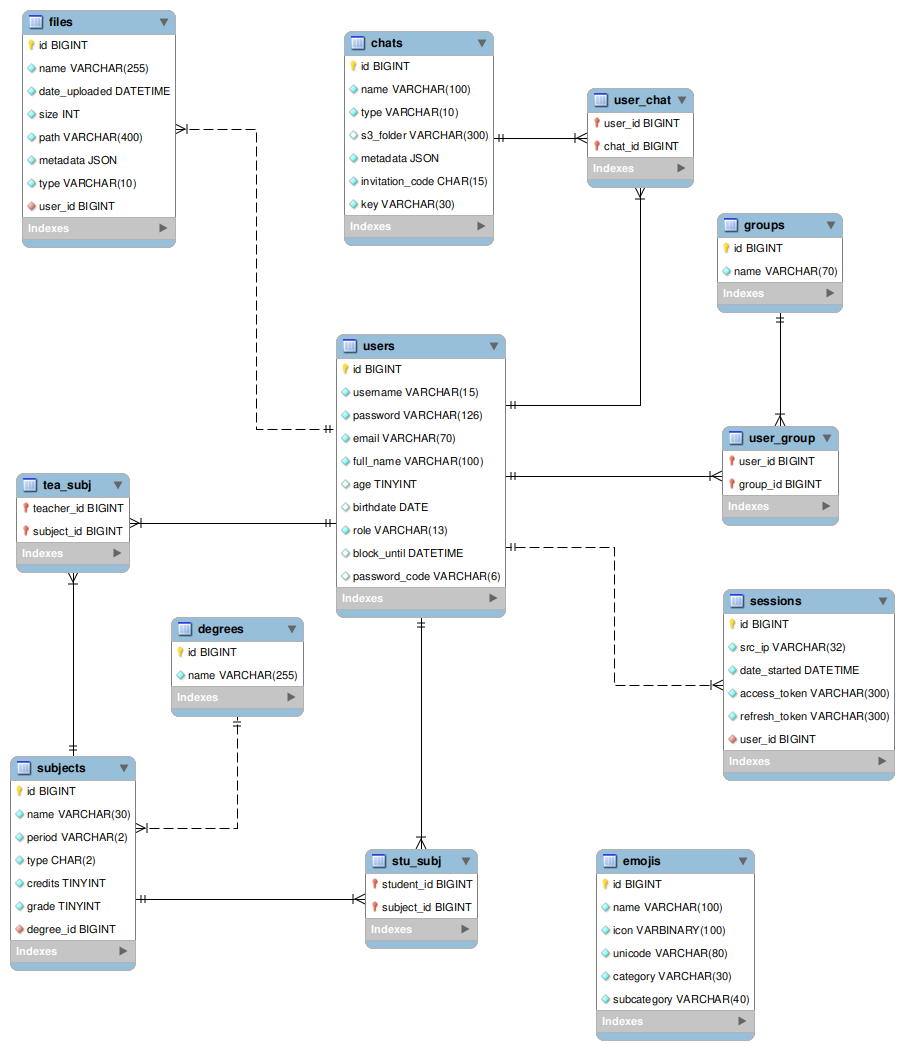
\includegraphics[width=0.8\textwidth]{diagramaBD}
	\caption{Diagrama de las tablas de la base de datos}
	\label{fig:diagrama-tablas}
\end{figure}

\sect{Seguridad}{seguridad}

Para la prevención de ciberataques al servidor por parte de usuarios malintencionados, se han
establecido las medidas de seguridad que se detallan a continuación:

\begin{itemize}
	\item \textbf{Cifrado de la comunicación entre el servidor y los clientes}: Para evitar que los datos de los
	usuarios puedan ser interceptados por terceros, se ha establecido un cifrado de las comunicaciones.\ Para ello, se
	ha empleado el protocolo TLS, que permite cifrar la comunicación utilizando el certificado SSL que proporciona
	Let's Encrypt.\ Este certificado se ha generado automáticamente mediante su servicio gratuito de certificados y,
	utilizando la aplicación \texttt{Certbot}, se renueva automáticamente cada 90 días.\ El certificado se
	almacena en el servidor en el directorio \texttt{/etc/letsencrypt/live/}.

	\item \textbf{Configuración del servidor ssh}: Para evitar que los usuarios puedan acceder al servidor mediante
	ssh, se ha configurado para que únicamente se pueda acceder mediante claves ssh (no permitiendo usuario y
	contraseña).\ Estas claves se obtienen mediante el comando \texttt{ssh-keygen}, que genera un par de claves
	(pública y privada), y se ha copiado la clave pública del cliente en el fichero
	\texttt{/home/user/.ssh/authorized\_keys} del servidor.\ De esta forma, únicamente se puede acceder al servidor
	mediante la
	clave privada del cliente.

	\item \textbf{Configuración del servidor web}: Se ha limitado la redirección de puertos desde el router hasta el
	servidor web, de forma que únicamente se puede acceder a los siguientes puertos:

	\begin{itemize}
		\item \boldFont{22}: puerto de ssh.
		\item \boldFont{80}: puerto de http.
		\item \boldFont{4040}: puerto de la aplicación en entorno de producción.
		\item \boldFont{4041}: puerto de la base de datos de la aplicación.
		\item \boldFont{4042}: puerto del servicio NSFW\@.
		\item \boldFont{4046}: puerto del panel de administración de Grafana.
	\end{itemize}

	Además, se ha configurado el servidor web para que únicamente se pueda acceder mediante el protocolo
	https, y no mediante http, haciendo que los usuarios sean redirigidos automáticamente a https.

	\item \textbf{Configuración de la base de datos}: La base de datos solo es accesible desde el propio servidor web,
	por lo que el acceso está restringido a la red interna.\ Para poder conectarse a la base de datos desde el
	exterior, se debe utilizar la clave ssh del servidor web, de forma que se accede a este y, desde ahí, se
	puede acceder a la base de datos.
\end{itemize}

\sect{Pruebas}{pruebas}



		\chaptr{Estado del arte}{estado-del-arte}
\sect{Aplicaciones similares}{aplicaciones-similares}

Se ha realizado una búsqueda de diferentes sitios web y aplicaciones que permitan la comunicación entre usuarios a
través de un chat en tiempo real, para determinar las funcionalidades generales que ofrecen y poder tomar una decisión
sobre las nuevas funcionalidades que se implementarán en la aplicación.\ La búsqueda se ha realizado en diferentes
idiomas (español e inglés) y se han encontrado diferentes páginas web y aplicaciones que ofrecen este tipo de
servicio, que son las siguientes:

\begin{itemize}
	\item \textbf{Chateagratis.net}: Esta página web permite a los usuarios elegir un apodo (que se escoge antes de
	iniciar las conversaciones) con el que entrar en el chat, por lo que no es necesaria la creación de una cuenta de
	usuario (aunque sí que se disponga de esta funcionalidad).\ La aplicación se divide en diferentes salas, cada una
	de las cuales tiene una temática diferente y se pueden mantener múltiples salas abiertas al mismo tiempo.\ Los
	usuarios pueden unirse a las salas existentes en un listado, disponible al acceder a la aplicación o en la pestaña
	asignada para ello.\ La página web permite a los usuarios enviar solamente mensajes de texto (con ciertos
	formatos, como negrita, colores, etc.) y emoticonos, sin la posibilidad de adjuntar imágenes o archivos.\ Se pueden
	programar bots para que administren una sala y que envíen mensajes automáticos cada cierto tiempo (como el que
	se visualiza en las siguientes imágenes, designado con el prefijo @).

	\begin{figure}[H]
		\centering
		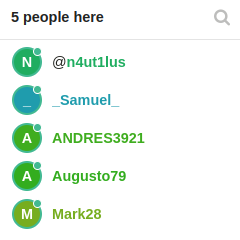
\includegraphics[scale=0.45]{ListaUsuariosChateagratis}
		\caption{Lista de usuarios conectados en una sala de chateagratis.net. (Fuente:~\cite{chateagratis:online}).}
		\label{fig:ListaUsuariosChateagratis}
	\end{figure}

	\begin{figure}[H]
		\centering
		
\includegraphics[scale=0.5]{ServerInfoMsgChateagratis}
		\caption{Mensajes de información del servidor en una sala de chat de chateagratis.net.
			(Fuente:~\cite{chateagratis:online}).}
		\label{fig:ServerInfoMsgChateagratis}
	\end{figure}

	\item \textbf{Dalechatea.me}: Esta página ofrece las mismas funciones que la anterior, pero con dos diferencias: se
	puede modificar el tamaño del chat (ancho y alto) para adaptarlo a la pantalla y necesidades del usuario y se
	pueden mandar archivos multimedia temporales (imágenes, vídeos y audios), que se borran pasados 15 minutos.
	Esta funcionalidad solo está disponible en los chats privados, no en los públicos.
	Además, se pueden agregar amigos, bloquear usuarios y añadir reacciones a mensajes de otros usuarios (como mandar
	un saludo o añadir a marcadores), entre otras funciones.

	\begin{figure}[H]
		\centering
		\raisebox{-0.4\height}{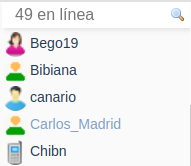
\includegraphics[scale=0.6]{ListaUsuariosDalechatea}}
		\hspace{1.5cm}
		
\includegraphics[scale=0.6]{InfoDalechatea}
		\caption{Lista de usuarios conectados y mensaje de información en una sala de chat de dalechatea.me.
			(Fuente:~\cite{DaleChat:online}).}
		\label{fig:UsuariosEInfoDalechatea}
	\end{figure}

	\item \textbf{Chatsfriends.com}: Esta página web ofrece las mismas funcionalidades que las anteriores, pero
	con un diseño renovado y diferente.\ Además, en la parte inferior (donde se escribe el mensaje) se muestra
	el nombre del usuario que será mostrado cuando se envíe el mensaje.\ A continuación se muestra una imagen
	de la página web, en la que se puede observar el chat en la parte central de la pantalla y un listado de
	usuarios en la parte derecha.

	\begin{figure}[H]
		\centering
		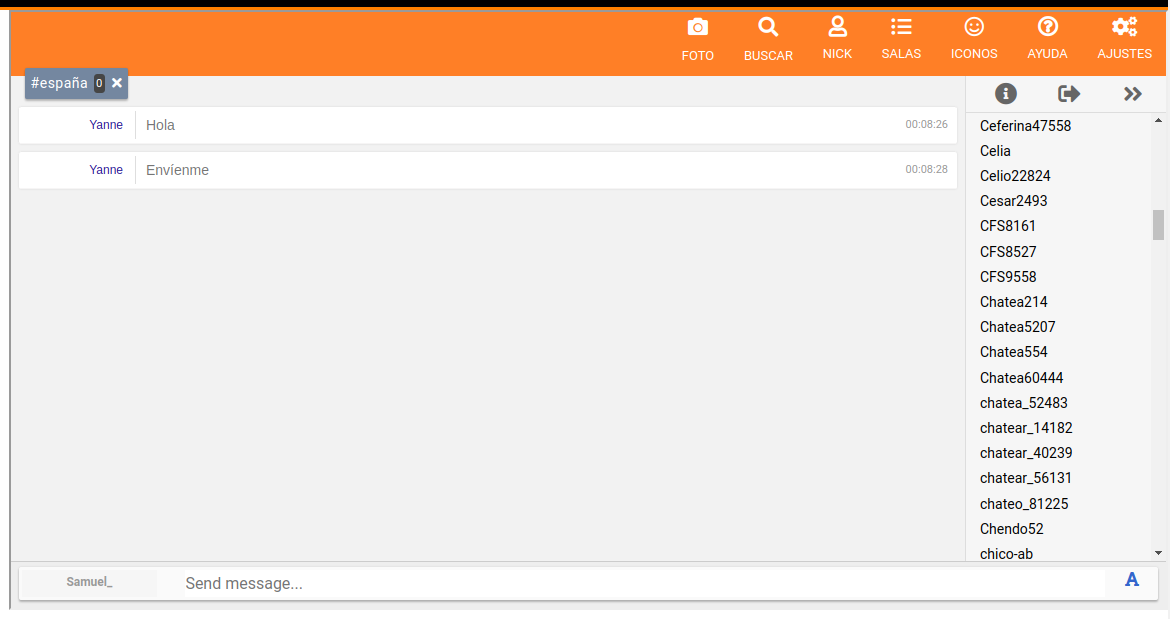
\includegraphics[width=0.8\textwidth]{Chatsfriends}
		\caption{Chat de la página web de chatsfriends.com. (Fuente:~\cite{chatsfriends:online}).}
		\label{fig:Chatsfriends}
	\end{figure}
\end{itemize}
\label{itm:estadoDelArte}

Todas las páginas tienen un diseño similar, con el chat en la parte central de la pantalla y un listado de usuarios
en la parte derecha (ver imagen~\ref{fig:chatCompleto}).\ La página web de chateagratis.net tiene un diseño más
sencillo y minimalista, mientras que la de dalechatea.me tiene un diseño más moderno y con más funcionalidades.
Ambos tienen un sistema de mensajes de información, que se envían por parte del servidor del chat, para notificar a
todos los usuarios conectados al mismo de cualquier evento.\ Cuando se hace clic en un usuario de la lista, se
muestra un pequeño popup con la información del usuario seleccionado, que muestra su nombre de usuario y ciertos
botones para realizar las acciones previamente mencionadas.

% Además, en la parte inferior de la ventana de información del usuario se muestra un listado de los últimos mensajes
% enviados por el usuario seleccionado.
% Chats a los que pertenece el usuario.

\begin{figure}[H]
	\centering
	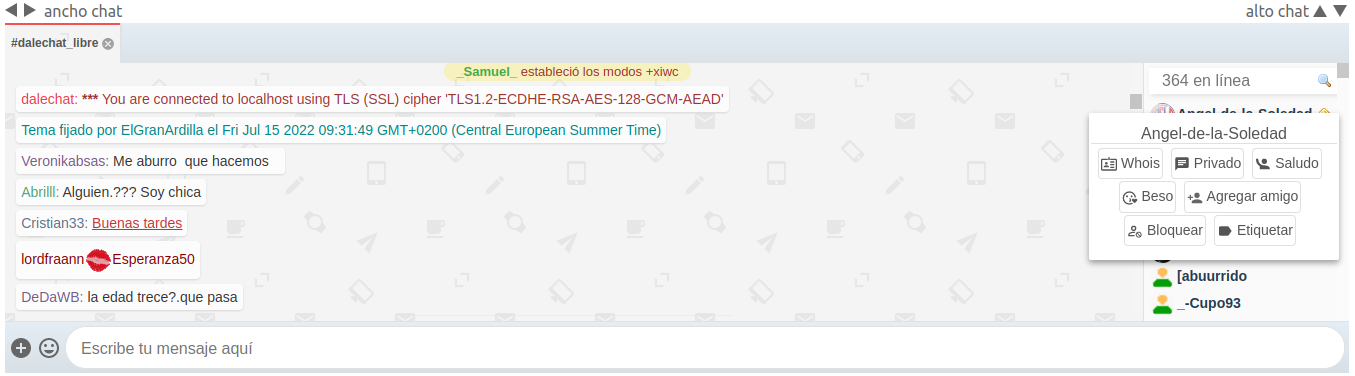
\includegraphics[scale=0.32]{Dalechatea}
	\caption{Chat completo de la página web de dalechatea.me. (Fuente:~\cite{DaleChat:online}).}
	\label{fig:chatCompleto}
\end{figure}


\sect{Opinión sobre el estado del arte}{opinion-sobre-el-estado-del-arte}

Haciendo una comparación entre las diferentes páginas web presentadas en la sección anterior, se
observa que ninguna de ellas dispone de las siguientes funcionalidades: un sistema de notificación auditiva
de mensajes recibidos, creación de grupos de chat personalizados y la posibilidad de enviar archivos
multimedia en los chats públicos.

\begin{itemize}
	\item \textbf{Notificación de mensajes}: En estas páginas web, cuando un usuario recibe un mensaje, no se le
	notifica de forma inmediata, sino que debe estar atento al chat para ver si aparece un mensaje nuevo.
	Esto puede ser molesto para los usuarios que no pueden prestar atención a la aplicación durante todo el
	tiempo que están conectados.\ Por ello, se ha decidido implementar un sistema de notificación de mensajes,
	que alerte al usuario cuando recibe un mensaje, de forma que pueda continuar con sus tareas sin tener que
	estar pendiente de la pantalla.

	\item \textbf{Creación de grupos de chat}: En la mayoría de las páginas web y aplicaciones de chat, los usuarios
	pueden unirse a salas de chat públicas, pero no pueden crear salas privadas.\ Esto puede no ser de agrado
	para algunos usuarios, que no pueden crear grupos de chat personalizados para comunicarse con sus amigos o
	familiares.\ Por ello, se ha decidido implementar un sistema de creación de grupos de chat, que permita a
	todos los usuarios crear grupos de chat personalizados para comunicarse con las personas que deseen.

	\item \textbf{Envío de archivos multimedia en los chats públicos}: En estas páginas web
	de chat, los usuarios pueden enviar distintos tipos de archivos multimedia en los chats privados, pero no en
	los públicos.\ Esto puede no satisfacer a todos los usuarios, ya que limita la comunicación entre los usuarios en
	los chats públicos.\ Por ello, se ha decidido implementar en todos los chats (ya sean públicos o privados) un
	sistema de envío de archivos multimedia.

	\item \textbf{Filtrado de imágenes inapropiadas}: En estas páginas web, los usuarios pueden enviar imágenes
	de cualquier tipo, incluyendo pornografía y otros contenidos inapropiados.\ Esto puede ser una molestia para
	la mayoría de los usuarios, que no quieren ver este tipo de imágenes.\ Por ello, se ha decidido implementar
	un sistema de filtrado de este tipo de contenido y que impida su envío en los chats.
	Además, cuando un usuario envíe un cierto número de imágenes pornográficas, se le bloqueará el acceso a la
	aplicación durante un tiempo determinado.
\end{itemize}

		\chaptr{Contenido}{contenido}
\sect{Patrones de diseño utilizados}{design-patterns}

Definición: \textit{Se trata de una solución que se puede aplicar a diferentes contextos y que se
puede reutilizar en diferentes proyectos.} \\

En este proyecto se han utilizado varios patrones de diseño, para permitir una mejor escalabilidad, mantenibilidad y
reutilización del código.\ A continuación se detallan los patrones utilizados y su justificación.

\subsect{Builder}{builder}


\subsect{Singleton}{singleton}
Este patrón se utiliza para garantizar que una clase tenga una única instancia y proporciona un punto de acceso
global a ella~\cite{sarcar2018java}.\ En el contexto de esta aplicación, se utiliza en ciertas
clases de utilidad y en las clases que asocian rutas a un método HTTP (por ejemplo \mono{/login} con el método POST).
Estas últimas son clases internas de \mono{Routes.java} y los nombres dependen del método HTTP que se debe utilizar para
realizar una petición a una ruta específica.

\begin{table}[ht]
	\centering
	\label{tab:routes}
	\begin{tabular}{|c|c|}
		\hline
		Método HTTP & Clase de la ruta   \\
		\hline
		GET           & \mono{GetRoute}    \\
		POST          & \mono{PostRoute}   \\
		PUT           & \mono{PutRoute}    \\
		DELETE        & \mono{DeleteRoute} \\
		\hline
	\end{tabular}
	\caption{Relación entre ruta y clase HTTP}
\end{table}

%\begin{lstlisting}[label={lst:lstlisting}]
%public class Routes {
%	private Routes() {
%	}
%	...
%	public static class GetRoute {
%	    public static final GetRoute INSTANCE = new GetRoute();
%		private GetRoute() {
%		}
%		public static final String USERS_URL = V_1 + "/users";
%		...
%	}
%	...
%}
%\end{lstlisting}

Código
\begin{minted}{c}
int main() {
	printf("hello, world");
	return 0;
}
\end{minted}

\subsect{Strategy}{strategy}


\sect{Procesamiento de los mensajes}{procesamiento-mensajes}

Como hemos visto en la sección anterior, los mensajes que se reciben en el servidor pueden ser de diferentes tipos,
cambiando la forma en que se procesan.\ A continuación se muestra una lista con las acciones que se realizan para
cada tipo de mensaje que se trata:

\begin{itemize}
	\item \boldFont{Text, Image, Video y Audio}: se envían al resto de usuarios del chat en el mismo formato en que llegaron al
	servidor.\ Estos cuatro tipos de mensaje contienen texto exclusivamente, siendo un mensaje o el enlace a un
	archivo almacenado en el bucket de S3.
	\item \boldFont{ActiveUsers}: se envía solo al cliente que lo ha solicitado, y contiene una lista con los usuarios que están
	conectados en ese momento al chat, ordenados alfabéticamente.
	\item \boldFont{GetHistory}: se envía al usuario que lo solicita, y contiene una lista con los últimos 65 mensajes que se han
	enviado al chat.\ Se realiza una lectura del fichero de texto que contiene el historial de mensajes (almacenado
	en disco) y un filtrado de los mensajes de actividad (los 2 siguientes) del solicitante, ya que no son relevantes.
	\item \boldFont{UserJoined y UserLeft}: se notifica a las personas conectadas el nombre del usuario que se ha unido o ha
	salido del chat, % todo (implementar): y se envía a todos los usuarios la lista de usuarios conectados actualizada.
	\item \boldFont{Ping}: se envía un mensaje con un breve texto.\ Se utiliza exclusivamente para mantener la conexión WebSocket
	abierta.
\end{itemize}

\sect{Ciclo de vida de la conexión de usuarios}{ciclo-de-vida-conexión-usuario}

Cuando un usuario accede a un chat de la aplicación, se inicia una conexión entre el cliente y el servidor a través
del protocolo de comunicación bidireccional \boldFont{WebSocket}~\cite{RFCWebSocket}.\ Esta conexión se mantiene
abierta mientras el
usuario esté en el chat, y se cierra cuando el usuario lo abandona.\ La secuencia de eventos que ocurren durante
la conexión de un usuario al chat es la siguiente:

\subsect{Frontend}{frontend}

\begin{enumerate}
	\item Se realiza una solicitud de conexión WebSocket al servidor.
	\item Se realiza una petición HTTP para comprobar que el usuario puede acceder al chat.\ Esto se realiza para
	que, en caso de que el usuario introduzca la URL de un chat al que no tiene acceso de forma manual, se le redirija
	a la página de inicio de la aplicación.
	\item Si se confirma que el usuario \boldFont{puede acceder} al chat:
	\begin{enumerate}
		\item Se establece la conexión WebSocket.
		\item Se envía un mensaje de tipo \monoFont{USER\_JOINED} al servidor.
		\item Se consultan los últimos mensajes del historial de mensajes del chat con el mensaje de tipo
		\monoFont{GET\_HISTORY\_MESSAGE}.
		\item Se realiza una petición de la lista de usuarios activos con un mensaje de tipo
		\monoFont{ACTIVE\_USERS\_MESSAGE}.
		\item Se configura un temporizador para mandar un mensaje de tipo \monoFont{PING\_MESSAGE} cada 30 segundos.
		Esto se realiza para que el servidor no cierre la conexión por inactividad.
	\end{enumerate}
	\item Si el usuario \boldFont{no puede acceder} al chat:
	\begin{enumerate}
		\item Se cierra la conexión WebSocket, en caso de llegarse a abrir.
		\item Se redirige al usuario a la página principal.
	\end{enumerate}
\end{enumerate}
\label{itm:frontend-connection-life-cycle}

\subsect{Backend}{backend}

Cuando comienza la ejecución del programa, se indica a Spring Boot que el manejador de mensajes a través de WebSocket
del servidor es una instancia de la clase \monoFont{WebSocketHandler}, en la ruta
\quoted{/ws/rschat}.\ Al instanciar esta clase, se crea un objeto \boldFont{chatMap} de tipo
\monoFont{WebSocketChatMap}, que contiene el atributo
\monoFont{chats} (ver Diagrama UML~\ref{diagram-WebSocketChatMapClass}).\ Es una tabla de dispersión que contiene los
chats activos en la aplicación.\ Cada entrada asocia a una cadena de texto (identificador del chat) la instancia de
un objeto de tipo \monoFont{Chat}.\ El proceso de \boldFont{conexión} al servidor sigue el siguiente flujo de eventos:

\begin{enumerate}
	\item Se establece la conexión WebSocket con el usuario.\ Esto ocurre de forma transparente al programador debido a
	que la implementación se realiza en el framework de Spring Boot.
	\item Se recibe el mensaje \monoFont{USER\_JOINED} del cliente y se crea un objeto de tipo \monoFont{WSClient}
	(formado por la instancia de \monoFont{WebSocketSession} y el \monoFont{WSClientID} del usuario).\ Este nuevo
	objeto se añade a la lista de usuarios conectados al chat.
	\begin{enumerate}
		\item Si el usuario es el primero que se ha conectado al chat, se crea uno nuevo, guardándose en la lista de
		chats.
		\item Si no, se añade al chat correspondiente de la lista de chats.
	\end{enumerate}
	\item Se recibe el mensaje \monoFont{GET\_HISTORY\_MESSAGE} del cliente y se envían como respuesta los últimos 65
	mensajes del historial de mensajes del chat.
	\item Se recibe el mensaje \monoFont{ACTIVE\_USERS\_MESSAGE} del cliente y se devuelve la lista con los usuarios
	activos en el chat.
\end{enumerate}
\label{itm:backend-connection-life-cycle}
Y el proceso de \boldFont{desconexión} se realiza como sigue:

\begin{enumerate}
	\item Se recibe el mensaje \monoFont{USER\_LEFT} del cliente.
	\item Se informa al resto de los usuarios del chat de la desconexión del usuario.
	\item Al eliminar un usuario del chat se pueden dar 2 casos:
	\begin{enumerate}
		\item Si el usuario es el último que se ha desconectado del chat, se elimina el chat de la tabla de dispersión
		\monoFont{chats}.\ Cuando esto ocurre, el historial de mensajes del chat que se haya registrado desde que se
		inició, se envía al almacenamiento en la nube.
		\item Si no, se elimina el usuario de la lista de usuarios del chat.
	\end{enumerate}
	\item Se cierra la conexión WebSocket con el usuario, de forma transparente al programador (al igual que la
	conexión).
\end{enumerate}

\begin{umlDiagram}
	\centering

	\begin{tikzpicture}
		\umlclass{WebSocketChatMap}{
			-- Map~<String, Chat>~ chats
		}{
			-- createChat(String): void \\
			-- chatExists(String): boolean \\
			-- getClientsOf(String): List~<WSClient> \\
			-- saveMessage(String, String): void \\
			+ getClient(WSClientID): WSClient \\
			+ addClientToChat(WSClient): void \\
			+ removeClientFromChat(WSClientID): void \\
			+ broadcastToSingleChat(String, String): void \\
			+ broadcastToSingleChatAndExcludeClient(WSClientID, String): void \\
			+ totalBroadcast(String): void \\
			+ getUsernamesOfChat(String): List~<String> \\
			-- saveAllToS3(): void \\
			-- deleteNullUsers(): void
		}{}
		\umlnote[y=-5.5,width=8.5cm]{WebSocketChatMap}{
			Los dos últimos métodos se ejecutan de manera periódica cada 10 y 3 minutos respectivamente.
		}{}
	\end{tikzpicture}

	\caption{Clase \monoFont{Chat} para almacenar los usuarios activos}
	\label{diagram-WebSocketChatMapClass}
\end{umlDiagram}

% Loki docker plugin causes all the containers to be unable to restart or kill. The alternative is to use the
% json-file driver with custom options. The json-file driver is the default driver for Docker.
% https://stackoverflow.com/questions/38567355/docker-compose-global-level-logging
% https://howchoo.com/devops/how-to-add-a-health-check-to-your-docker-container

\sect{Docker}{docker}
Docker es una plataforma software que permite el desarrollo, prueba y ejecución de aplicaciones de forma rápida y
cómoda, separando la aplicación de la infraestructura permitiendo ejecutar múltiples aplicaciones en un mismo servidor
(ver imagen~\ref{fig:docker-container-infrastructure}).\ Esto se realiza empaquetando la
aplicación, sus dependencias y otras herramientas necesarias para su ejecución en lo que se denominan
\boldFont{contenedores}, que son instancias ejecutables de una imagen de Docker.\ Las imágenes son ficheros de solo
lectura que contienen las instrucciones necesarias para crear un contenedor y normalmente se basan en otras imágenes
añadiendo o modificando configuraciones~\cite{docker-docs}.

\begin{figure}[ht]
	\centering
	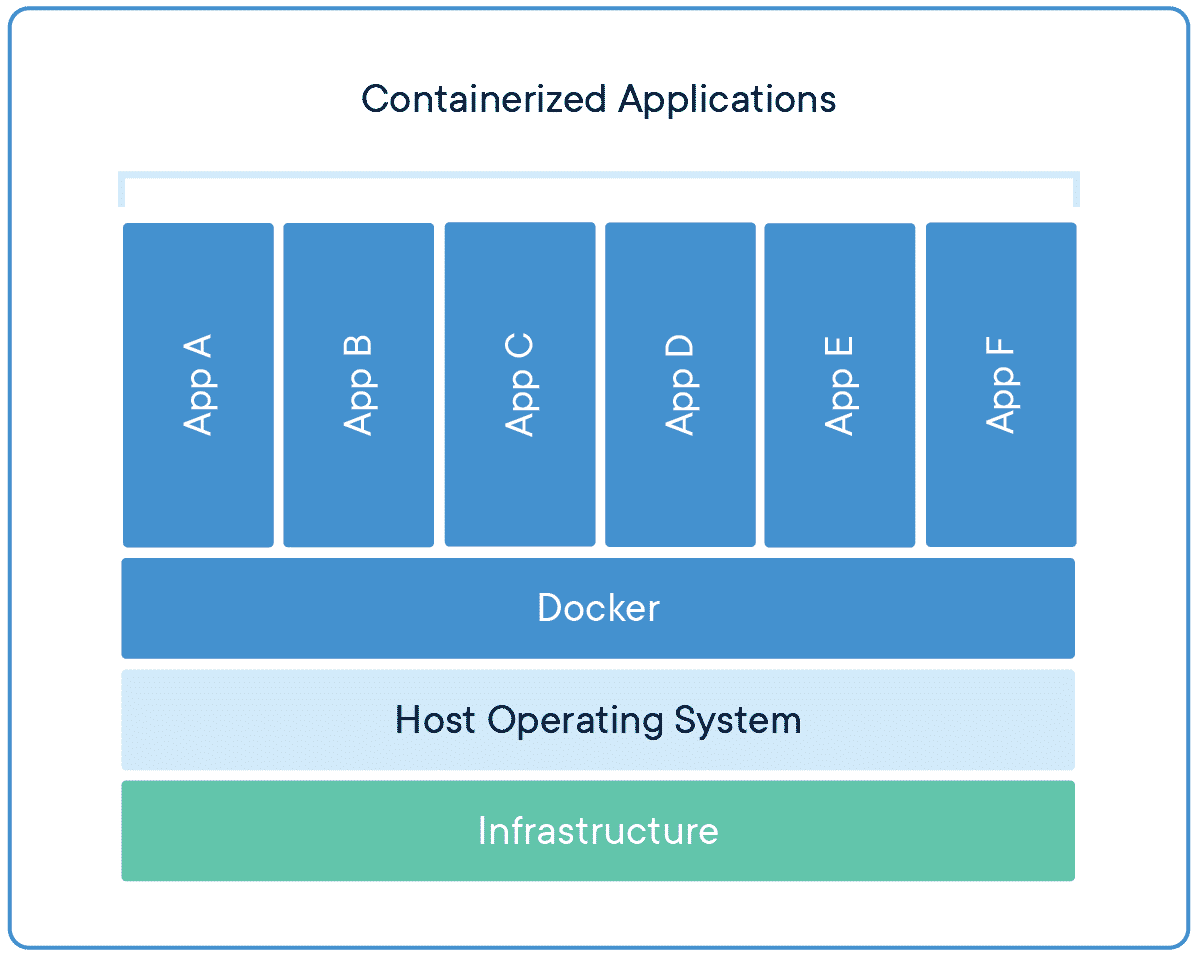
\includegraphics[width=0.8\textwidth]{res/images/container-what-is-container}
	\caption{Infrastructura docker. Fuente: \url{https://www.docker.com/resources/what-container}}
	\label{fig:docker-container-infrastructure}
\end{figure}

En el desarrollo de la aplicación se ha utilizado Docker para la creación de una imagen que contenga todo el código de
la aplicación así como las variables de entorno necesarias para su correcto funcionamiento.\ Se ha
utilizado la herramienta \monoFont{docker-compose}, que permite definir y ejecutar contenedores Docker de manera
sencilla.\ Para la configuración de los contenedores, se dispone del fichero \monoFont{docker-compose.yml} que se
encuentra en la raíz del proyecto y define los servicios que se ejecutarán en los contenedores, así como
las dependencias entre ellos.

Debido a que cada vez que se elimina un contenedor (al reiniciar el sistema o al generar de nuevo la imagen de la
aplicación para incluir cambios del código) se pierden los datos, la persistencia de los mismos y de sus
configuraciones es necesaria.\ Para lograr esto, se usan \boldFont{volúmenes}, que son directorios creados y
gestionados por Docker que se almacenan en el sistema de archivos del host, y que se montan en los contenedores cuando
se inicializan~\cite{docker-volumes}.\ De esta forma, los datos no se pierden al eliminar el contenedor.\ Los
volúmenes se definen en el mismo fichero \monoFont{docker-compose.yml} mediante la opción \monoFont{volumes} y son
los siguientes:

\begin{itemize}
	\item \monoFont{rschat-db}: contiene los datos y script inicial de la base de datos.
	\item \monoFont{rschat-logs}: contiene los ficheros de registro de la aplicación.
	\item \monoFont{grafana-storage}: contiene la configuración de Grafana.
\end{itemize}

A continuación, se mencionan todos los contenedores utilizados para la aplicación junto con una breve descripción de
cada uno de ellos:

	{\scriptsize Nota: los marcados con el símbolo \textsuperscript{\textasteriskcentered} se describirán en detalle
más adelante.}

\begin{itemize}
	\item \monoFont{rschat}: Contenedor que ejecuta el backend de la aplicación.
	\item \monoFont{rschat-db}: Contenedor que ejecuta la base de datos MySQL\@.
	\item \monoFont{prometheus\textsuperscript{\textasteriskcentered}}: Contenedor que ejecuta el servidor de métricas
	de Prometheus.
	\item \monoFont{grafana\textsuperscript{\textasteriskcentered}}: Contenedor que ejecuta el panel de observabilidad
	de Grafana.
	\item \monoFont{loki\textsuperscript{\textasteriskcentered}}: Contenedor que ejecuta el servidor de logs Loki.
	\item \monoFont{promtail\textsuperscript{\textasteriskcentered}}: Contenedor que ejecuta el agente de logs
	Promtail.
\end{itemize}
\label{itm:docker-compose-services}

\subsect{Prometheus (Métricas)}{prometheus}
Prometheus es un conjunto de herramientas de código abierto para la \boldFont{monitorización} de sistemas y
\boldFont{alertas} que recoge y
almacena las métricas con la marca de tiempo cuando se producen, incluyendo etiquetas (clave-valor) de manera
opcional~\cite{prometheus-overview}.
Estas métricas se utilizan para determinar el funcionamiento y estado de la aplicación en tiempo real, permitiendo
diagnosticar problemas de rendimiento o recursos de una manera rápida y sencilla.\ Para habilitar la exportación de
las métricas (de manera automática) por parte de la aplicación hay que realizar ciertas configuraciones,
que se detallan a continuación:

\begin{itemize}
	\item Añadir 2 librerías en el fichero \monoFont{pom.xml}~\cite{prometheus-metrics-pom}:
	\begin{itemize}
		\item spring-boot-starter-actuator
		\item micrometer-registry-prometheus
	\end{itemize}

	\item Para exponer el \quoted{endpoint} que permite ver las métricas, hay que añadir una propiedad en el fichero
	\monoFont{application.properties}:
	\begin{itemize}
		\item \monoFont{management.endpoints.web.exposure.include=prometheus}
	\end{itemize}

	\item Permitir las peticiones de tipo GET a \monoFont{/actuator/prometheus}: esto se configura
	de manera programática estableciendo la ruta como pública (permitiendo peticiones GET sin necesidad de estar
	autenticado).
\end{itemize}
\label{itm:metrics-export-config}

Las métricas que más se utilizarán son las relacionadas con el rendimiento de la aplicación y el uso de recursos del
sistema, aunque se han añadido algunas personalizadas para determinar el uso que se hace de determinadas partes de la
aplicación.\ La lista con las métricas más usadas es la siguiente:

\begin{itemize}
	\item jvm\_memory\_used\_bytes: bytes usados por la JVM\@.
	\item jvm\_memory\_committed\_bytes: bytes que se están guardando en el \quoted{heap} de la JVM\@.
	\item system\_cpu\_usage: uso de CPU del sistema.
	\item process\_cpu\_usage: uso de CPU por parte de la aplicación.
	\item system\_cpu\_count: número de procesadores físicos utilizados en todo el sistema.
	\item logback\_events\_total: número de eventos de log de un determinado nivel (info, debug, warn, error).
	\item http\_server\_requests\_seconds\_count: número de peticiones HTTP realizadas a la aplicación.
	\item jvm\_threads\_live\_threads: número de hilos en ejecución.
	\item jvm\_threads\_daemon\_threads: número de hilos en ejecución (en segundo plano).
	\item jvm\_threads\_peak\_threads: número máximo de hilos.
\end{itemize}
\label{itm:most-used-metrics}


\subsect{Grafana (Panel de observabilidad)}{grafana}

\subsect{Loki (Servidor de logs)}{loki}

\subsect{Promtail (Agente de logs)}{promtail}

\sect{Base de datos}{base-datos}

El sistema gestor de base de datos utilizado para la aplicación es \monoFont{MySQL}.\ Las bases de datos de MySQL son
relacionales, lo que significa que los datos se almacenan en tablas, que están formadas por filas (campos) y columnas
(registros).\ Las tablas se relacionan entre sí mediante claves primarias y claves foráneas, que son campos que
identifican a cada registro de la tabla.
% Todo: esto es un poco básico, ¿se pone?
Este tipo de base de datos es muy empleado en aplicaciones web, por lo que es sencillo encontrar información sobre
cómo usar MySQL\@.\ Como el lenguaje de programación con el que se ha desarrollado el backend de la aplicación es
Java, se ha utilizado el ORM \monoFont{Hibernate}, que permite realizar un mapeado de la base de datos a objetos de
Java, de forma que se puede trabajar con ella de una forma transparente y cómoda para el programador.\ Para realizar
las operaciones de inserción, actualización, consulta y borrado de los datos, \monoFont{Spring Boot Data JPA} es la
mejor opción, ya que se encarga de realizar estas operaciones de forma transparente para el desarrollador,
dependiendo del nombre que reciba un método.\ También, mediante el uso de anotaciones (expresiones precedidas por el
símbolo @, como por ejemplo \monoFont{@Query}), se pueden personalizar de las consultas que se ejecutarán en base de
datos.\ El diagrama de las tablas de la base de datos de la aplicación se muestra en la siguiente figura:

\begin{figure}[H]
	\centering
	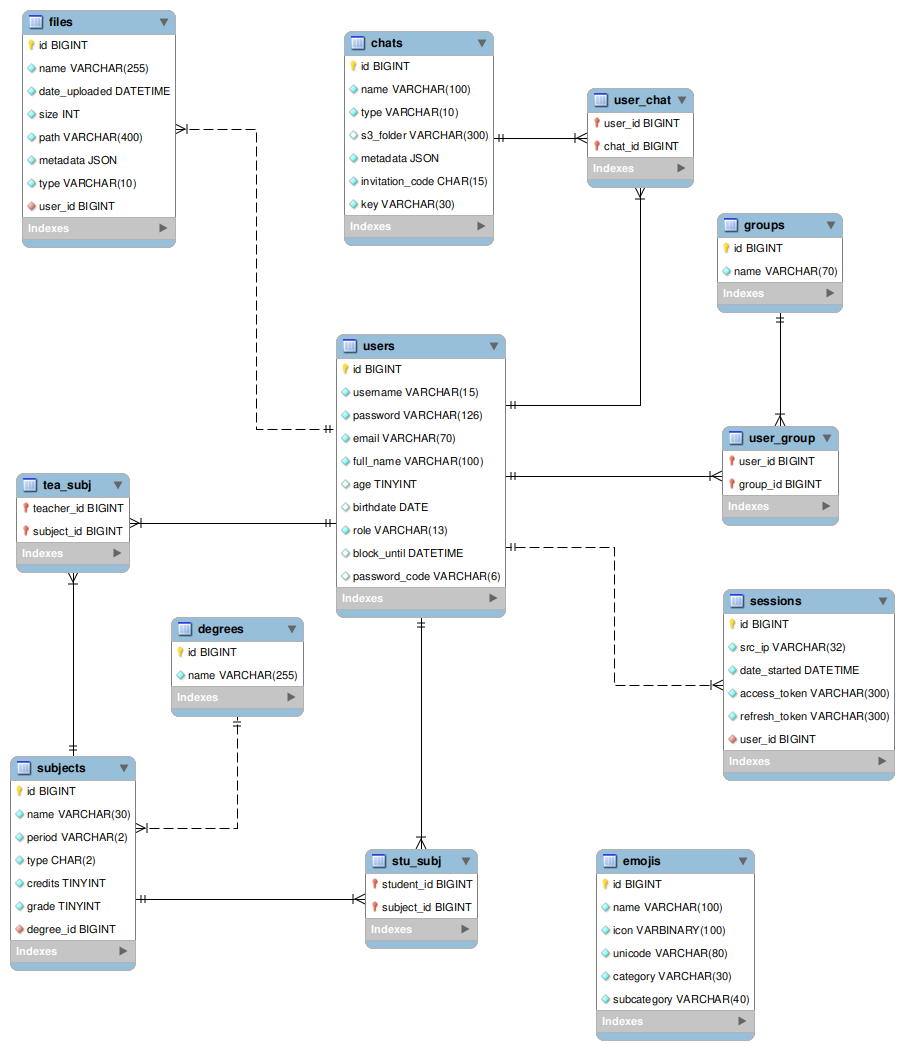
\includegraphics[width=0.8\textwidth]{diagramaBD}
	\caption{Diagrama de las tablas de la base de datos}
	\label{fig:diagrama-tablas}
\end{figure}

\sect{Seguridad}{seguridad}

Para la prevención de ciberataques al servidor por parte de usuarios malintencionados, se han
establecido las medidas de seguridad que se detallan a continuación:

\begin{itemize}
	\item \textbf{Cifrado de la comunicación entre el servidor y los clientes}: Para evitar que los datos de los
	usuarios puedan ser interceptados por terceros, se ha establecido un cifrado de las comunicaciones.\ Para ello, se
	ha empleado el protocolo TLS, que permite cifrar la comunicación utilizando el certificado SSL que proporciona
	Let's Encrypt.\ Este certificado se ha generado automáticamente mediante su servicio gratuito de certificados y,
	utilizando la aplicación \texttt{Certbot}, se renueva automáticamente cada 90 días.\ El certificado se
	almacena en el servidor en el directorio \texttt{/etc/letsencrypt/live/}.

	\item \textbf{Configuración del servidor ssh}: Para evitar que los usuarios puedan acceder al servidor mediante
	ssh, se ha configurado para que únicamente se pueda acceder mediante claves ssh (no permitiendo usuario y
	contraseña).\ Estas claves se obtienen mediante el comando \texttt{ssh-keygen}, que genera un par de claves
	(pública y privada), y se ha copiado la clave pública del cliente en el fichero
	\texttt{/home/user/.ssh/authorized\_keys} del servidor.\ De esta forma, únicamente se puede acceder al servidor
	mediante la
	clave privada del cliente.

	\item \textbf{Configuración del servidor web}: Se ha limitado la redirección de puertos desde el router hasta el
	servidor web, de forma que únicamente se puede acceder a los siguientes puertos:

	\begin{itemize}
		\item \boldFont{22}: puerto de ssh.
		\item \boldFont{80}: puerto de http.
		\item \boldFont{4040}: puerto de la aplicación en entorno de producción.
		\item \boldFont{4041}: puerto de la base de datos de la aplicación.
		\item \boldFont{4042}: puerto del servicio NSFW\@.
		\item \boldFont{4046}: puerto del panel de administración de Grafana.
	\end{itemize}

	Además, se ha configurado el servidor web para que únicamente se pueda acceder mediante el protocolo
	https, y no mediante http, haciendo que los usuarios sean redirigidos automáticamente a https.

	\item \textbf{Configuración de la base de datos}: La base de datos solo es accesible desde el propio servidor web,
	por lo que el acceso está restringido a la red interna.\ Para poder conectarse a la base de datos desde el
	exterior, se debe utilizar la clave ssh del servidor web, de forma que se accede a este y, desde ahí, se
	puede acceder a la base de datos.
\end{itemize}

\sect{Pruebas}{pruebas}


\sect{Patrones de diseño utilizados}{design-patterns}

Definición: \textit{Se trata de una solución que se puede aplicar a diferentes contextos y que se
puede reutilizar en diferentes proyectos.} \\

En este proyecto se han utilizado varios patrones de diseño, para permitir una mejor escalabilidad, mantenibilidad y
reutilización del código.\ A continuación se detallan los patrones utilizados y su justificación.

\subsect{Builder}{builder}


\subsect{Singleton}{singleton}
Este patrón se utiliza para garantizar que una clase tenga una única instancia y proporciona un punto de acceso
global a ella~\cite{sarcar2018java}.\ En el contexto de esta aplicación, se utiliza en ciertas
clases de utilidad y en las clases que asocian rutas a un método HTTP (por ejemplo \mono{/login} con el método POST).
Estas últimas son clases internas de \mono{Routes.java} y los nombres dependen del método HTTP que se debe utilizar para
realizar una petición a una ruta específica.

\begin{table}[ht]
	\centering
	\label{tab:routes}
	\begin{tabular}{|c|c|}
		\hline
		Método HTTP & Clase de la ruta   \\
		\hline
		GET           & \mono{GetRoute}    \\
		POST          & \mono{PostRoute}   \\
		PUT           & \mono{PutRoute}    \\
		DELETE        & \mono{DeleteRoute} \\
		\hline
	\end{tabular}
	\caption{Relación entre ruta y clase HTTP}
\end{table}

%\begin{lstlisting}[label={lst:lstlisting}]
%public class Routes {
%	private Routes() {
%	}
%	...
%	public static class GetRoute {
%	    public static final GetRoute INSTANCE = new GetRoute();
%		private GetRoute() {
%		}
%		public static final String USERS_URL = V_1 + "/users";
%		...
%	}
%	...
%}
%\end{lstlisting}

Código
\begin{minted}{c}
int main() {
	printf("hello, world");
	return 0;
}
\end{minted}

\subsect{Strategy}{strategy}


\sect{Procesamiento de los mensajes}{procesamiento-mensajes}

Como hemos visto en la sección anterior, los mensajes que se reciben en el servidor pueden ser de diferentes tipos,
cambiando la forma en que se procesan.\ A continuación se muestra una lista con las acciones que se realizan para
cada tipo de mensaje que se trata:

\begin{itemize}
	\item \boldFont{Text, Image, Video y Audio}: se envían al resto de usuarios del chat en el mismo formato en que llegaron al
	servidor.\ Estos cuatro tipos de mensaje contienen texto exclusivamente, siendo un mensaje o el enlace a un
	archivo almacenado en el bucket de S3.
	\item \boldFont{ActiveUsers}: se envía solo al cliente que lo ha solicitado, y contiene una lista con los usuarios que están
	conectados en ese momento al chat, ordenados alfabéticamente.
	\item \boldFont{GetHistory}: se envía al usuario que lo solicita, y contiene una lista con los últimos 65 mensajes que se han
	enviado al chat.\ Se realiza una lectura del fichero de texto que contiene el historial de mensajes (almacenado
	en disco) y un filtrado de los mensajes de actividad (los 2 siguientes) del solicitante, ya que no son relevantes.
	\item \boldFont{UserJoined y UserLeft}: se notifica a las personas conectadas el nombre del usuario que se ha unido o ha
	salido del chat, % todo (implementar): y se envía a todos los usuarios la lista de usuarios conectados actualizada.
	\item \boldFont{Ping}: se envía un mensaje con un breve texto.\ Se utiliza exclusivamente para mantener la conexión WebSocket
	abierta.
\end{itemize}

\sect{Ciclo de vida de la conexión de usuarios}{ciclo-de-vida-conexión-usuario}

Cuando un usuario accede a un chat de la aplicación, se inicia una conexión entre el cliente y el servidor a través
del protocolo de comunicación bidireccional \boldFont{WebSocket}~\cite{RFCWebSocket}.\ Esta conexión se mantiene
abierta mientras el
usuario esté en el chat, y se cierra cuando el usuario lo abandona.\ La secuencia de eventos que ocurren durante
la conexión de un usuario al chat es la siguiente:

\subsect{Frontend}{frontend}

\begin{enumerate}
	\item Se realiza una solicitud de conexión WebSocket al servidor.
	\item Se realiza una petición HTTP para comprobar que el usuario puede acceder al chat.\ Esto se realiza para
	que, en caso de que el usuario introduzca la URL de un chat al que no tiene acceso de forma manual, se le redirija
	a la página de inicio de la aplicación.
	\item Si se confirma que el usuario \boldFont{puede acceder} al chat:
	\begin{enumerate}
		\item Se establece la conexión WebSocket.
		\item Se envía un mensaje de tipo \monoFont{USER\_JOINED} al servidor.
		\item Se consultan los últimos mensajes del historial de mensajes del chat con el mensaje de tipo
		\monoFont{GET\_HISTORY\_MESSAGE}.
		\item Se realiza una petición de la lista de usuarios activos con un mensaje de tipo
		\monoFont{ACTIVE\_USERS\_MESSAGE}.
		\item Se configura un temporizador para mandar un mensaje de tipo \monoFont{PING\_MESSAGE} cada 30 segundos.
		Esto se realiza para que el servidor no cierre la conexión por inactividad.
	\end{enumerate}
	\item Si el usuario \boldFont{no puede acceder} al chat:
	\begin{enumerate}
		\item Se cierra la conexión WebSocket, en caso de llegarse a abrir.
		\item Se redirige al usuario a la página principal.
	\end{enumerate}
\end{enumerate}
\label{itm:frontend-connection-life-cycle}

\subsect{Backend}{backend}

Cuando comienza la ejecución del programa, se indica a Spring Boot que el manejador de mensajes a través de WebSocket
del servidor es una instancia de la clase \monoFont{WebSocketHandler}, en la ruta
\quoted{/ws/rschat}.\ Al instanciar esta clase, se crea un objeto \boldFont{chatMap} de tipo
\monoFont{WebSocketChatMap}, que contiene el atributo
\monoFont{chats} (ver Diagrama UML~\ref{diagram-WebSocketChatMapClass}).\ Es una tabla de dispersión que contiene los
chats activos en la aplicación.\ Cada entrada asocia a una cadena de texto (identificador del chat) la instancia de
un objeto de tipo \monoFont{Chat}.\ El proceso de \boldFont{conexión} al servidor sigue el siguiente flujo de eventos:

\begin{enumerate}
	\item Se establece la conexión WebSocket con el usuario.\ Esto ocurre de forma transparente al programador debido a
	que la implementación se realiza en el framework de Spring Boot.
	\item Se recibe el mensaje \monoFont{USER\_JOINED} del cliente y se crea un objeto de tipo \monoFont{WSClient}
	(formado por la instancia de \monoFont{WebSocketSession} y el \monoFont{WSClientID} del usuario).\ Este nuevo
	objeto se añade a la lista de usuarios conectados al chat.
	\begin{enumerate}
		\item Si el usuario es el primero que se ha conectado al chat, se crea uno nuevo, guardándose en la lista de
		chats.
		\item Si no, se añade al chat correspondiente de la lista de chats.
	\end{enumerate}
	\item Se recibe el mensaje \monoFont{GET\_HISTORY\_MESSAGE} del cliente y se envían como respuesta los últimos 65
	mensajes del historial de mensajes del chat.
	\item Se recibe el mensaje \monoFont{ACTIVE\_USERS\_MESSAGE} del cliente y se devuelve la lista con los usuarios
	activos en el chat.
\end{enumerate}
\label{itm:backend-connection-life-cycle}
Y el proceso de \boldFont{desconexión} se realiza como sigue:

\begin{enumerate}
	\item Se recibe el mensaje \monoFont{USER\_LEFT} del cliente.
	\item Se informa al resto de los usuarios del chat de la desconexión del usuario.
	\item Al eliminar un usuario del chat se pueden dar 2 casos:
	\begin{enumerate}
		\item Si el usuario es el último que se ha desconectado del chat, se elimina el chat de la tabla de dispersión
		\monoFont{chats}.\ Cuando esto ocurre, el historial de mensajes del chat que se haya registrado desde que se
		inició, se envía al almacenamiento en la nube.
		\item Si no, se elimina el usuario de la lista de usuarios del chat.
	\end{enumerate}
	\item Se cierra la conexión WebSocket con el usuario, de forma transparente al programador (al igual que la
	conexión).
\end{enumerate}

\begin{umlDiagram}
	\centering

	\begin{tikzpicture}
		\umlclass{WebSocketChatMap}{
			-- Map~<String, Chat>~ chats
		}{
			-- createChat(String): void \\
			-- chatExists(String): boolean \\
			-- getClientsOf(String): List~<WSClient> \\
			-- saveMessage(String, String): void \\
			+ getClient(WSClientID): WSClient \\
			+ addClientToChat(WSClient): void \\
			+ removeClientFromChat(WSClientID): void \\
			+ broadcastToSingleChat(String, String): void \\
			+ broadcastToSingleChatAndExcludeClient(WSClientID, String): void \\
			+ totalBroadcast(String): void \\
			+ getUsernamesOfChat(String): List~<String> \\
			-- saveAllToS3(): void \\
			-- deleteNullUsers(): void
		}{}
		\umlnote[y=-5.5,width=8.5cm]{WebSocketChatMap}{
			Los dos últimos métodos se ejecutan de manera periódica cada 10 y 3 minutos respectivamente.
		}{}
	\end{tikzpicture}

	\caption{Clase \monoFont{Chat} para almacenar los usuarios activos}
	\label{diagram-WebSocketChatMapClass}
\end{umlDiagram}

% Loki docker plugin causes all the containers to be unable to restart or kill. The alternative is to use the
% json-file driver with custom options. The json-file driver is the default driver for Docker.
% https://stackoverflow.com/questions/38567355/docker-compose-global-level-logging
% https://howchoo.com/devops/how-to-add-a-health-check-to-your-docker-container

\sect{Docker}{docker}
Docker es una plataforma software que permite el desarrollo, prueba y ejecución de aplicaciones de forma rápida y
cómoda, separando la aplicación de la infraestructura permitiendo ejecutar múltiples aplicaciones en un mismo servidor
(ver imagen~\ref{fig:docker-container-infrastructure}).\ Esto se realiza empaquetando la
aplicación, sus dependencias y otras herramientas necesarias para su ejecución en lo que se denominan
\boldFont{contenedores}, que son instancias ejecutables de una imagen de Docker.\ Las imágenes son ficheros de solo
lectura que contienen las instrucciones necesarias para crear un contenedor y normalmente se basan en otras imágenes
añadiendo o modificando configuraciones~\cite{docker-docs}.

\begin{figure}[ht]
	\centering
	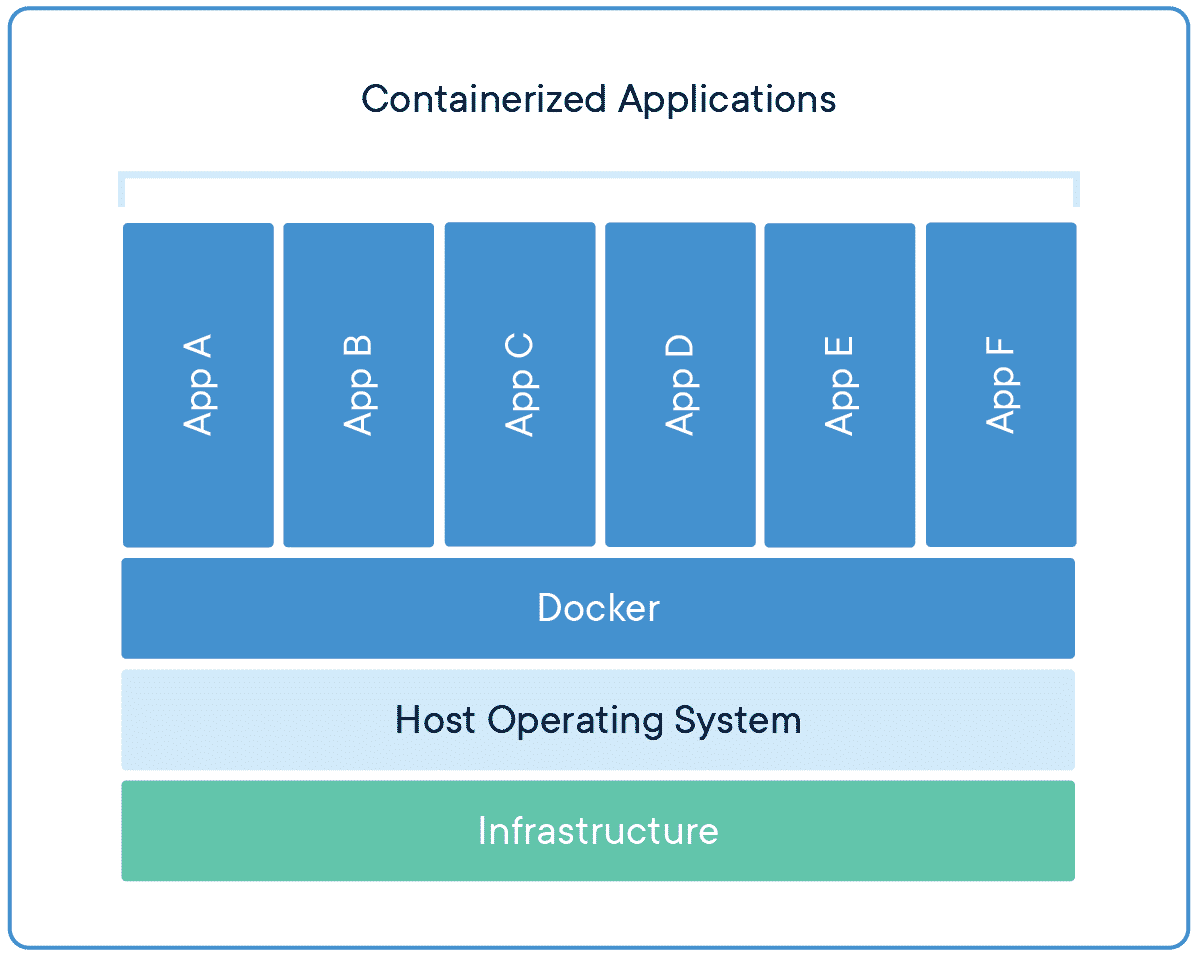
\includegraphics[width=0.8\textwidth]{res/images/container-what-is-container}
	\caption{Infrastructura docker. Fuente: \url{https://www.docker.com/resources/what-container}}
	\label{fig:docker-container-infrastructure}
\end{figure}

En el desarrollo de la aplicación se ha utilizado Docker para la creación de una imagen que contenga todo el código de
la aplicación así como las variables de entorno necesarias para su correcto funcionamiento.\ Se ha
utilizado la herramienta \monoFont{docker-compose}, que permite definir y ejecutar contenedores Docker de manera
sencilla.\ Para la configuración de los contenedores, se dispone del fichero \monoFont{docker-compose.yml} que se
encuentra en la raíz del proyecto y define los servicios que se ejecutarán en los contenedores, así como
las dependencias entre ellos.

Debido a que cada vez que se elimina un contenedor (al reiniciar el sistema o al generar de nuevo la imagen de la
aplicación para incluir cambios del código) se pierden los datos, la persistencia de los mismos y de sus
configuraciones es necesaria.\ Para lograr esto, se usan \boldFont{volúmenes}, que son directorios creados y
gestionados por Docker que se almacenan en el sistema de archivos del host, y que se montan en los contenedores cuando
se inicializan~\cite{docker-volumes}.\ De esta forma, los datos no se pierden al eliminar el contenedor.\ Los
volúmenes se definen en el mismo fichero \monoFont{docker-compose.yml} mediante la opción \monoFont{volumes} y son
los siguientes:

\begin{itemize}
	\item \monoFont{rschat-db}: contiene los datos y script inicial de la base de datos.
	\item \monoFont{rschat-logs}: contiene los ficheros de registro de la aplicación.
	\item \monoFont{grafana-storage}: contiene la configuración de Grafana.
\end{itemize}

A continuación, se mencionan todos los contenedores utilizados para la aplicación junto con una breve descripción de
cada uno de ellos:

	{\scriptsize Nota: los marcados con el símbolo \textsuperscript{\textasteriskcentered} se describirán en detalle
más adelante.}

\begin{itemize}
	\item \monoFont{rschat}: Contenedor que ejecuta el backend de la aplicación.
	\item \monoFont{rschat-db}: Contenedor que ejecuta la base de datos MySQL\@.
	\item \monoFont{prometheus\textsuperscript{\textasteriskcentered}}: Contenedor que ejecuta el servidor de métricas
	de Prometheus.
	\item \monoFont{grafana\textsuperscript{\textasteriskcentered}}: Contenedor que ejecuta el panel de observabilidad
	de Grafana.
	\item \monoFont{loki\textsuperscript{\textasteriskcentered}}: Contenedor que ejecuta el servidor de logs Loki.
	\item \monoFont{promtail\textsuperscript{\textasteriskcentered}}: Contenedor que ejecuta el agente de logs
	Promtail.
\end{itemize}
\label{itm:docker-compose-services}

\subsect{Prometheus (Métricas)}{prometheus}
Prometheus es un conjunto de herramientas de código abierto para la \boldFont{monitorización} de sistemas y
\boldFont{alertas} que recoge y
almacena las métricas con la marca de tiempo cuando se producen, incluyendo etiquetas (clave-valor) de manera
opcional~\cite{prometheus-overview}.
Estas métricas se utilizan para determinar el funcionamiento y estado de la aplicación en tiempo real, permitiendo
diagnosticar problemas de rendimiento o recursos de una manera rápida y sencilla.\ Para habilitar la exportación de
las métricas (de manera automática) por parte de la aplicación hay que realizar ciertas configuraciones,
que se detallan a continuación:

\begin{itemize}
	\item Añadir 2 librerías en el fichero \monoFont{pom.xml}~\cite{prometheus-metrics-pom}:
	\begin{itemize}
		\item spring-boot-starter-actuator
		\item micrometer-registry-prometheus
	\end{itemize}

	\item Para exponer el \quoted{endpoint} que permite ver las métricas, hay que añadir una propiedad en el fichero
	\monoFont{application.properties}:
	\begin{itemize}
		\item \monoFont{management.endpoints.web.exposure.include=prometheus}
	\end{itemize}

	\item Permitir las peticiones de tipo GET a \monoFont{/actuator/prometheus}: esto se configura
	de manera programática estableciendo la ruta como pública (permitiendo peticiones GET sin necesidad de estar
	autenticado).
\end{itemize}
\label{itm:metrics-export-config}

Las métricas que más se utilizarán son las relacionadas con el rendimiento de la aplicación y el uso de recursos del
sistema, aunque se han añadido algunas personalizadas para determinar el uso que se hace de determinadas partes de la
aplicación.\ La lista con las métricas más usadas es la siguiente:

\begin{itemize}
	\item jvm\_memory\_used\_bytes: bytes usados por la JVM\@.
	\item jvm\_memory\_committed\_bytes: bytes que se están guardando en el \quoted{heap} de la JVM\@.
	\item system\_cpu\_usage: uso de CPU del sistema.
	\item process\_cpu\_usage: uso de CPU por parte de la aplicación.
	\item system\_cpu\_count: número de procesadores físicos utilizados en todo el sistema.
	\item logback\_events\_total: número de eventos de log de un determinado nivel (info, debug, warn, error).
	\item http\_server\_requests\_seconds\_count: número de peticiones HTTP realizadas a la aplicación.
	\item jvm\_threads\_live\_threads: número de hilos en ejecución.
	\item jvm\_threads\_daemon\_threads: número de hilos en ejecución (en segundo plano).
	\item jvm\_threads\_peak\_threads: número máximo de hilos.
\end{itemize}
\label{itm:most-used-metrics}


\subsect{Grafana (Panel de observabilidad)}{grafana}

\subsect{Loki (Servidor de logs)}{loki}

\subsect{Promtail (Agente de logs)}{promtail}

\sect{Base de datos}{base-datos}

El sistema gestor de base de datos utilizado para la aplicación es \monoFont{MySQL}.\ Las bases de datos de MySQL son
relacionales, lo que significa que los datos se almacenan en tablas, que están formadas por filas (campos) y columnas
(registros).\ Las tablas se relacionan entre sí mediante claves primarias y claves foráneas, que son campos que
identifican a cada registro de la tabla.
% Todo: esto es un poco básico, ¿se pone?
Este tipo de base de datos es muy empleado en aplicaciones web, por lo que es sencillo encontrar información sobre
cómo usar MySQL\@.\ Como el lenguaje de programación con el que se ha desarrollado el backend de la aplicación es
Java, se ha utilizado el ORM \monoFont{Hibernate}, que permite realizar un mapeado de la base de datos a objetos de
Java, de forma que se puede trabajar con ella de una forma transparente y cómoda para el programador.\ Para realizar
las operaciones de inserción, actualización, consulta y borrado de los datos, \monoFont{Spring Boot Data JPA} es la
mejor opción, ya que se encarga de realizar estas operaciones de forma transparente para el desarrollador,
dependiendo del nombre que reciba un método.\ También, mediante el uso de anotaciones (expresiones precedidas por el
símbolo @, como por ejemplo \monoFont{@Query}), se pueden personalizar de las consultas que se ejecutarán en base de
datos.\ El diagrama de las tablas de la base de datos de la aplicación se muestra en la siguiente figura:

\begin{figure}[H]
	\centering
	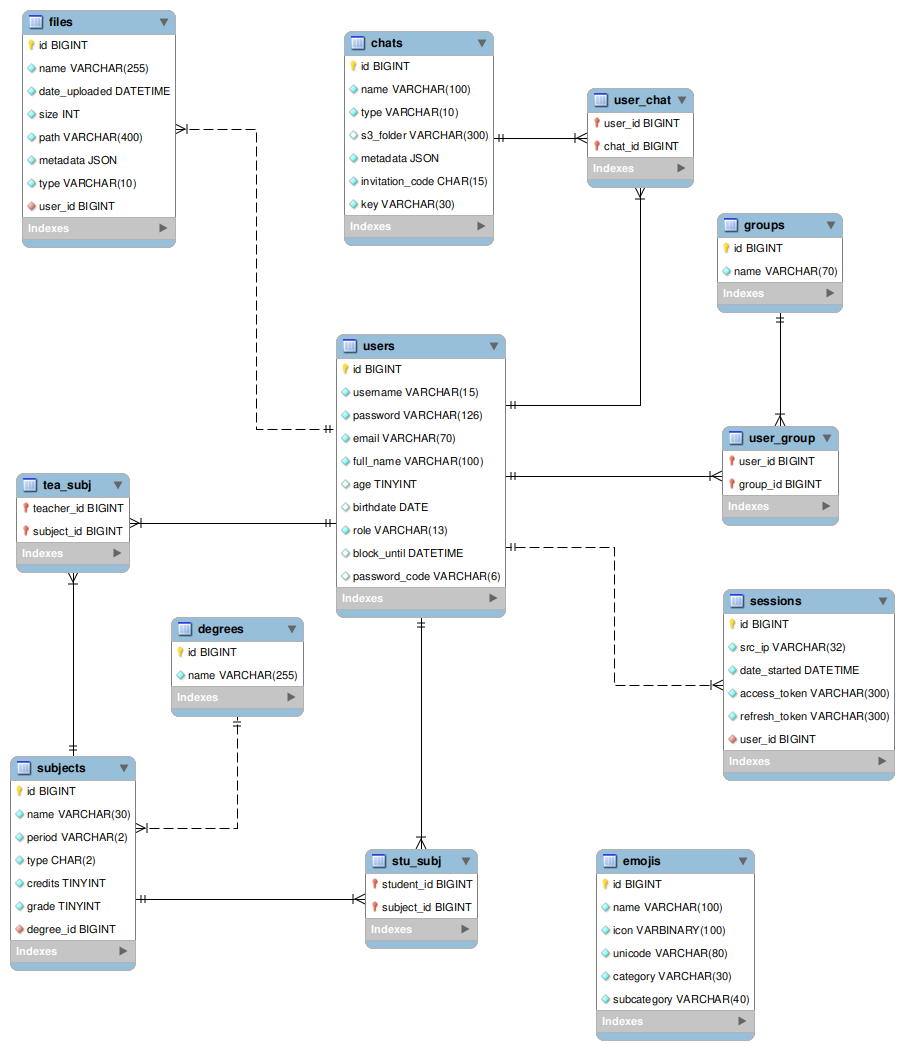
\includegraphics[width=0.8\textwidth]{diagramaBD}
	\caption{Diagrama de las tablas de la base de datos}
	\label{fig:diagrama-tablas}
\end{figure}

\sect{Seguridad}{seguridad}

Para la prevención de ciberataques al servidor por parte de usuarios malintencionados, se han
establecido las medidas de seguridad que se detallan a continuación:

\begin{itemize}
	\item \textbf{Cifrado de la comunicación entre el servidor y los clientes}: Para evitar que los datos de los
	usuarios puedan ser interceptados por terceros, se ha establecido un cifrado de las comunicaciones.\ Para ello, se
	ha empleado el protocolo TLS, que permite cifrar la comunicación utilizando el certificado SSL que proporciona
	Let's Encrypt.\ Este certificado se ha generado automáticamente mediante su servicio gratuito de certificados y,
	utilizando la aplicación \texttt{Certbot}, se renueva automáticamente cada 90 días.\ El certificado se
	almacena en el servidor en el directorio \texttt{/etc/letsencrypt/live/}.

	\item \textbf{Configuración del servidor ssh}: Para evitar que los usuarios puedan acceder al servidor mediante
	ssh, se ha configurado para que únicamente se pueda acceder mediante claves ssh (no permitiendo usuario y
	contraseña).\ Estas claves se obtienen mediante el comando \texttt{ssh-keygen}, que genera un par de claves
	(pública y privada), y se ha copiado la clave pública del cliente en el fichero
	\texttt{/home/user/.ssh/authorized\_keys} del servidor.\ De esta forma, únicamente se puede acceder al servidor
	mediante la
	clave privada del cliente.

	\item \textbf{Configuración del servidor web}: Se ha limitado la redirección de puertos desde el router hasta el
	servidor web, de forma que únicamente se puede acceder a los siguientes puertos:

	\begin{itemize}
		\item \boldFont{22}: puerto de ssh.
		\item \boldFont{80}: puerto de http.
		\item \boldFont{4040}: puerto de la aplicación en entorno de producción.
		\item \boldFont{4041}: puerto de la base de datos de la aplicación.
		\item \boldFont{4042}: puerto del servicio NSFW\@.
		\item \boldFont{4046}: puerto del panel de administración de Grafana.
	\end{itemize}

	Además, se ha configurado el servidor web para que únicamente se pueda acceder mediante el protocolo
	https, y no mediante http, haciendo que los usuarios sean redirigidos automáticamente a https.

	\item \textbf{Configuración de la base de datos}: La base de datos solo es accesible desde el propio servidor web,
	por lo que el acceso está restringido a la red interna.\ Para poder conectarse a la base de datos desde el
	exterior, se debe utilizar la clave ssh del servidor web, de forma que se accede a este y, desde ahí, se
	puede acceder a la base de datos.
\end{itemize}

\sect{Pruebas}{pruebas}


\sect{Patrones de diseño utilizados}{design-patterns}

Definición: \textit{Se trata de una solución que se puede aplicar a diferentes contextos y que se
puede reutilizar en diferentes proyectos.} \\

En este proyecto se han utilizado varios patrones de diseño, para permitir una mejor escalabilidad, mantenibilidad y
reutilización del código.\ A continuación se detallan los patrones utilizados y su justificación.

\subsect{Builder}{builder}


\subsect{Singleton}{singleton}
Este patrón se utiliza para garantizar que una clase tenga una única instancia y proporciona un punto de acceso
global a ella~\cite{sarcar2018java}.\ En el contexto de esta aplicación, se utiliza en ciertas
clases de utilidad y en las clases que asocian rutas a un método HTTP (por ejemplo \mono{/login} con el método POST).
Estas últimas son clases internas de \mono{Routes.java} y los nombres dependen del método HTTP que se debe utilizar para
realizar una petición a una ruta específica.

\begin{table}[ht]
	\centering
	\label{tab:routes}
	\begin{tabular}{|c|c|}
		\hline
		Método HTTP & Clase de la ruta   \\
		\hline
		GET           & \mono{GetRoute}    \\
		POST          & \mono{PostRoute}   \\
		PUT           & \mono{PutRoute}    \\
		DELETE        & \mono{DeleteRoute} \\
		\hline
	\end{tabular}
	\caption{Relación entre ruta y clase HTTP}
\end{table}

%\begin{lstlisting}[label={lst:lstlisting}]
%public class Routes {
%	private Routes() {
%	}
%	...
%	public static class GetRoute {
%	    public static final GetRoute INSTANCE = new GetRoute();
%		private GetRoute() {
%		}
%		public static final String USERS_URL = V_1 + "/users";
%		...
%	}
%	...
%}
%\end{lstlisting}

Código
\begin{minted}{c}
int main() {
	printf("hello, world");
	return 0;
}
\end{minted}

\subsect{Strategy}{strategy}


\sect{Procesamiento de los mensajes}{procesamiento-mensajes}

Como hemos visto en la sección anterior, los mensajes que se reciben en el servidor pueden ser de diferentes tipos,
cambiando la forma en que se procesan.\ A continuación se muestra una lista con las acciones que se realizan para
cada tipo de mensaje que se trata:

\begin{itemize}
	\item \boldFont{Text, Image, Video y Audio}: se envían al resto de usuarios del chat en el mismo formato en que llegaron al
	servidor.\ Estos cuatro tipos de mensaje contienen texto exclusivamente, siendo un mensaje o el enlace a un
	archivo almacenado en el bucket de S3.
	\item \boldFont{ActiveUsers}: se envía solo al cliente que lo ha solicitado, y contiene una lista con los usuarios que están
	conectados en ese momento al chat, ordenados alfabéticamente.
	\item \boldFont{GetHistory}: se envía al usuario que lo solicita, y contiene una lista con los últimos 65 mensajes que se han
	enviado al chat.\ Se realiza una lectura del fichero de texto que contiene el historial de mensajes (almacenado
	en disco) y un filtrado de los mensajes de actividad (los 2 siguientes) del solicitante, ya que no son relevantes.
	\item \boldFont{UserJoined y UserLeft}: se notifica a las personas conectadas el nombre del usuario que se ha unido o ha
	salido del chat, % todo (implementar): y se envía a todos los usuarios la lista de usuarios conectados actualizada.
	\item \boldFont{Ping}: se envía un mensaje con un breve texto.\ Se utiliza exclusivamente para mantener la conexión WebSocket
	abierta.
\end{itemize}

\sect{Ciclo de vida de la conexión de usuarios}{ciclo-de-vida-conexión-usuario}

Cuando un usuario accede a un chat de la aplicación, se inicia una conexión entre el cliente y el servidor a través
del protocolo de comunicación bidireccional \boldFont{WebSocket}~\cite{RFCWebSocket}.\ Esta conexión se mantiene
abierta mientras el
usuario esté en el chat, y se cierra cuando el usuario lo abandona.\ La secuencia de eventos que ocurren durante
la conexión de un usuario al chat es la siguiente:

\subsect{Frontend}{frontend}

\begin{enumerate}
	\item Se realiza una solicitud de conexión WebSocket al servidor.
	\item Se realiza una petición HTTP para comprobar que el usuario puede acceder al chat.\ Esto se realiza para
	que, en caso de que el usuario introduzca la URL de un chat al que no tiene acceso de forma manual, se le redirija
	a la página de inicio de la aplicación.
	\item Si se confirma que el usuario \boldFont{puede acceder} al chat:
	\begin{enumerate}
		\item Se establece la conexión WebSocket.
		\item Se envía un mensaje de tipo \monoFont{USER\_JOINED} al servidor.
		\item Se consultan los últimos mensajes del historial de mensajes del chat con el mensaje de tipo
		\monoFont{GET\_HISTORY\_MESSAGE}.
		\item Se realiza una petición de la lista de usuarios activos con un mensaje de tipo
		\monoFont{ACTIVE\_USERS\_MESSAGE}.
		\item Se configura un temporizador para mandar un mensaje de tipo \monoFont{PING\_MESSAGE} cada 30 segundos.
		Esto se realiza para que el servidor no cierre la conexión por inactividad.
	\end{enumerate}
	\item Si el usuario \boldFont{no puede acceder} al chat:
	\begin{enumerate}
		\item Se cierra la conexión WebSocket, en caso de llegarse a abrir.
		\item Se redirige al usuario a la página principal.
	\end{enumerate}
\end{enumerate}
\label{itm:frontend-connection-life-cycle}

\subsect{Backend}{backend}

Cuando comienza la ejecución del programa, se indica a Spring Boot que el manejador de mensajes a través de WebSocket
del servidor es una instancia de la clase \monoFont{WebSocketHandler}, en la ruta
\quoted{/ws/rschat}.\ Al instanciar esta clase, se crea un objeto \boldFont{chatMap} de tipo
\monoFont{WebSocketChatMap}, que contiene el atributo
\monoFont{chats} (ver Diagrama UML~\ref{diagram-WebSocketChatMapClass}).\ Es una tabla de dispersión que contiene los
chats activos en la aplicación.\ Cada entrada asocia a una cadena de texto (identificador del chat) la instancia de
un objeto de tipo \monoFont{Chat}.\ El proceso de \boldFont{conexión} al servidor sigue el siguiente flujo de eventos:

\begin{enumerate}
	\item Se establece la conexión WebSocket con el usuario.\ Esto ocurre de forma transparente al programador debido a
	que la implementación se realiza en el framework de Spring Boot.
	\item Se recibe el mensaje \monoFont{USER\_JOINED} del cliente y se crea un objeto de tipo \monoFont{WSClient}
	(formado por la instancia de \monoFont{WebSocketSession} y el \monoFont{WSClientID} del usuario).\ Este nuevo
	objeto se añade a la lista de usuarios conectados al chat.
	\begin{enumerate}
		\item Si el usuario es el primero que se ha conectado al chat, se crea uno nuevo, guardándose en la lista de
		chats.
		\item Si no, se añade al chat correspondiente de la lista de chats.
	\end{enumerate}
	\item Se recibe el mensaje \monoFont{GET\_HISTORY\_MESSAGE} del cliente y se envían como respuesta los últimos 65
	mensajes del historial de mensajes del chat.
	\item Se recibe el mensaje \monoFont{ACTIVE\_USERS\_MESSAGE} del cliente y se devuelve la lista con los usuarios
	activos en el chat.
\end{enumerate}
\label{itm:backend-connection-life-cycle}
Y el proceso de \boldFont{desconexión} se realiza como sigue:

\begin{enumerate}
	\item Se recibe el mensaje \monoFont{USER\_LEFT} del cliente.
	\item Se informa al resto de los usuarios del chat de la desconexión del usuario.
	\item Al eliminar un usuario del chat se pueden dar 2 casos:
	\begin{enumerate}
		\item Si el usuario es el último que se ha desconectado del chat, se elimina el chat de la tabla de dispersión
		\monoFont{chats}.\ Cuando esto ocurre, el historial de mensajes del chat que se haya registrado desde que se
		inició, se envía al almacenamiento en la nube.
		\item Si no, se elimina el usuario de la lista de usuarios del chat.
	\end{enumerate}
	\item Se cierra la conexión WebSocket con el usuario, de forma transparente al programador (al igual que la
	conexión).
\end{enumerate}

\begin{umlDiagram}
	\centering

	\begin{tikzpicture}
		\umlclass{WebSocketChatMap}{
			-- Map~<String, Chat>~ chats
		}{
			-- createChat(String): void \\
			-- chatExists(String): boolean \\
			-- getClientsOf(String): List~<WSClient> \\
			-- saveMessage(String, String): void \\
			+ getClient(WSClientID): WSClient \\
			+ addClientToChat(WSClient): void \\
			+ removeClientFromChat(WSClientID): void \\
			+ broadcastToSingleChat(String, String): void \\
			+ broadcastToSingleChatAndExcludeClient(WSClientID, String): void \\
			+ totalBroadcast(String): void \\
			+ getUsernamesOfChat(String): List~<String> \\
			-- saveAllToS3(): void \\
			-- deleteNullUsers(): void
		}{}
		\umlnote[y=-5.5,width=8.5cm]{WebSocketChatMap}{
			Los dos últimos métodos se ejecutan de manera periódica cada 10 y 3 minutos respectivamente.
		}{}
	\end{tikzpicture}

	\caption{Clase \monoFont{Chat} para almacenar los usuarios activos}
	\label{diagram-WebSocketChatMapClass}
\end{umlDiagram}

% Loki docker plugin causes all the containers to be unable to restart or kill. The alternative is to use the
% json-file driver with custom options. The json-file driver is the default driver for Docker.
% https://stackoverflow.com/questions/38567355/docker-compose-global-level-logging
% https://howchoo.com/devops/how-to-add-a-health-check-to-your-docker-container

\sect{Docker}{docker}
Docker es una plataforma software que permite el desarrollo, prueba y ejecución de aplicaciones de forma rápida y
cómoda, separando la aplicación de la infraestructura permitiendo ejecutar múltiples aplicaciones en un mismo servidor
(ver imagen~\ref{fig:docker-container-infrastructure}).\ Esto se realiza empaquetando la
aplicación, sus dependencias y otras herramientas necesarias para su ejecución en lo que se denominan
\boldFont{contenedores}, que son instancias ejecutables de una imagen de Docker.\ Las imágenes son ficheros de solo
lectura que contienen las instrucciones necesarias para crear un contenedor y normalmente se basan en otras imágenes
añadiendo o modificando configuraciones~\cite{docker-docs}.

\begin{figure}[ht]
	\centering
	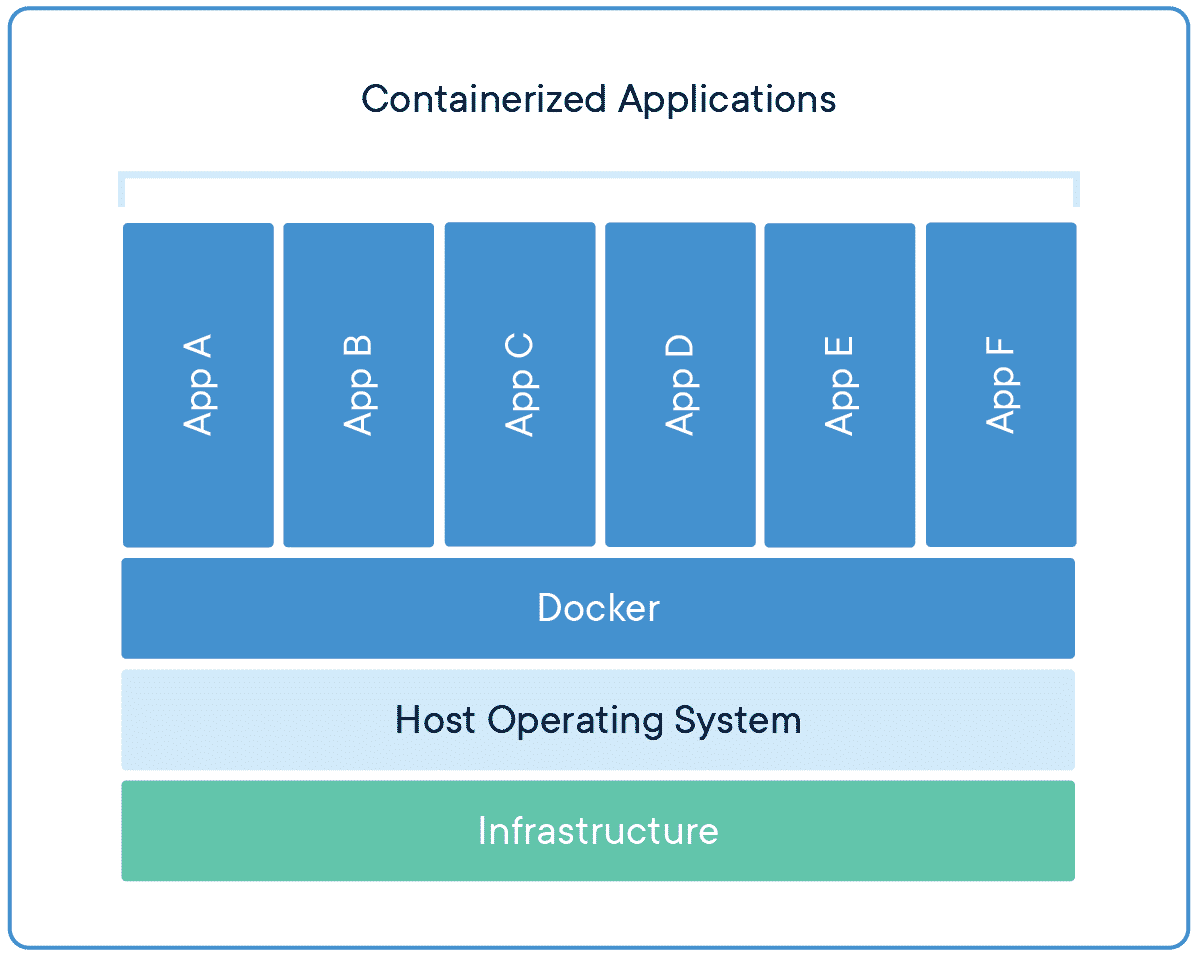
\includegraphics[width=0.8\textwidth]{res/images/container-what-is-container}
	\caption{Infrastructura docker. Fuente: \url{https://www.docker.com/resources/what-container}}
	\label{fig:docker-container-infrastructure}
\end{figure}

En el desarrollo de la aplicación se ha utilizado Docker para la creación de una imagen que contenga todo el código de
la aplicación así como las variables de entorno necesarias para su correcto funcionamiento.\ Se ha
utilizado la herramienta \monoFont{docker-compose}, que permite definir y ejecutar contenedores Docker de manera
sencilla.\ Para la configuración de los contenedores, se dispone del fichero \monoFont{docker-compose.yml} que se
encuentra en la raíz del proyecto y define los servicios que se ejecutarán en los contenedores, así como
las dependencias entre ellos.

Debido a que cada vez que se elimina un contenedor (al reiniciar el sistema o al generar de nuevo la imagen de la
aplicación para incluir cambios del código) se pierden los datos, la persistencia de los mismos y de sus
configuraciones es necesaria.\ Para lograr esto, se usan \boldFont{volúmenes}, que son directorios creados y
gestionados por Docker que se almacenan en el sistema de archivos del host, y que se montan en los contenedores cuando
se inicializan~\cite{docker-volumes}.\ De esta forma, los datos no se pierden al eliminar el contenedor.\ Los
volúmenes se definen en el mismo fichero \monoFont{docker-compose.yml} mediante la opción \monoFont{volumes} y son
los siguientes:

\begin{itemize}
	\item \monoFont{rschat-db}: contiene los datos y script inicial de la base de datos.
	\item \monoFont{rschat-logs}: contiene los ficheros de registro de la aplicación.
	\item \monoFont{grafana-storage}: contiene la configuración de Grafana.
\end{itemize}

A continuación, se mencionan todos los contenedores utilizados para la aplicación junto con una breve descripción de
cada uno de ellos:

	{\scriptsize Nota: los marcados con el símbolo \textsuperscript{\textasteriskcentered} se describirán en detalle
más adelante.}

\begin{itemize}
	\item \monoFont{rschat}: Contenedor que ejecuta el backend de la aplicación.
	\item \monoFont{rschat-db}: Contenedor que ejecuta la base de datos MySQL\@.
	\item \monoFont{prometheus\textsuperscript{\textasteriskcentered}}: Contenedor que ejecuta el servidor de métricas
	de Prometheus.
	\item \monoFont{grafana\textsuperscript{\textasteriskcentered}}: Contenedor que ejecuta el panel de observabilidad
	de Grafana.
	\item \monoFont{loki\textsuperscript{\textasteriskcentered}}: Contenedor que ejecuta el servidor de logs Loki.
	\item \monoFont{promtail\textsuperscript{\textasteriskcentered}}: Contenedor que ejecuta el agente de logs
	Promtail.
\end{itemize}
\label{itm:docker-compose-services}

\subsect{Prometheus (Métricas)}{prometheus}
Prometheus es un conjunto de herramientas de código abierto para la \boldFont{monitorización} de sistemas y
\boldFont{alertas} que recoge y
almacena las métricas con la marca de tiempo cuando se producen, incluyendo etiquetas (clave-valor) de manera
opcional~\cite{prometheus-overview}.
Estas métricas se utilizan para determinar el funcionamiento y estado de la aplicación en tiempo real, permitiendo
diagnosticar problemas de rendimiento o recursos de una manera rápida y sencilla.\ Para habilitar la exportación de
las métricas (de manera automática) por parte de la aplicación hay que realizar ciertas configuraciones,
que se detallan a continuación:

\begin{itemize}
	\item Añadir 2 librerías en el fichero \monoFont{pom.xml}~\cite{prometheus-metrics-pom}:
	\begin{itemize}
		\item spring-boot-starter-actuator
		\item micrometer-registry-prometheus
	\end{itemize}

	\item Para exponer el \quoted{endpoint} que permite ver las métricas, hay que añadir una propiedad en el fichero
	\monoFont{application.properties}:
	\begin{itemize}
		\item \monoFont{management.endpoints.web.exposure.include=prometheus}
	\end{itemize}

	\item Permitir las peticiones de tipo GET a \monoFont{/actuator/prometheus}: esto se configura
	de manera programática estableciendo la ruta como pública (permitiendo peticiones GET sin necesidad de estar
	autenticado).
\end{itemize}
\label{itm:metrics-export-config}

Las métricas que más se utilizarán son las relacionadas con el rendimiento de la aplicación y el uso de recursos del
sistema, aunque se han añadido algunas personalizadas para determinar el uso que se hace de determinadas partes de la
aplicación.\ La lista con las métricas más usadas es la siguiente:

\begin{itemize}
	\item jvm\_memory\_used\_bytes: bytes usados por la JVM\@.
	\item jvm\_memory\_committed\_bytes: bytes que se están guardando en el \quoted{heap} de la JVM\@.
	\item system\_cpu\_usage: uso de CPU del sistema.
	\item process\_cpu\_usage: uso de CPU por parte de la aplicación.
	\item system\_cpu\_count: número de procesadores físicos utilizados en todo el sistema.
	\item logback\_events\_total: número de eventos de log de un determinado nivel (info, debug, warn, error).
	\item http\_server\_requests\_seconds\_count: número de peticiones HTTP realizadas a la aplicación.
	\item jvm\_threads\_live\_threads: número de hilos en ejecución.
	\item jvm\_threads\_daemon\_threads: número de hilos en ejecución (en segundo plano).
	\item jvm\_threads\_peak\_threads: número máximo de hilos.
\end{itemize}
\label{itm:most-used-metrics}


\subsect{Grafana (Panel de observabilidad)}{grafana}

\subsect{Loki (Servidor de logs)}{loki}

\subsect{Promtail (Agente de logs)}{promtail}

\sect{Base de datos}{base-datos}

El sistema gestor de base de datos utilizado para la aplicación es \monoFont{MySQL}.\ Las bases de datos de MySQL son
relacionales, lo que significa que los datos se almacenan en tablas, que están formadas por filas (campos) y columnas
(registros).\ Las tablas se relacionan entre sí mediante claves primarias y claves foráneas, que son campos que
identifican a cada registro de la tabla.
% Todo: esto es un poco básico, ¿se pone?
Este tipo de base de datos es muy empleado en aplicaciones web, por lo que es sencillo encontrar información sobre
cómo usar MySQL\@.\ Como el lenguaje de programación con el que se ha desarrollado el backend de la aplicación es
Java, se ha utilizado el ORM \monoFont{Hibernate}, que permite realizar un mapeado de la base de datos a objetos de
Java, de forma que se puede trabajar con ella de una forma transparente y cómoda para el programador.\ Para realizar
las operaciones de inserción, actualización, consulta y borrado de los datos, \monoFont{Spring Boot Data JPA} es la
mejor opción, ya que se encarga de realizar estas operaciones de forma transparente para el desarrollador,
dependiendo del nombre que reciba un método.\ También, mediante el uso de anotaciones (expresiones precedidas por el
símbolo @, como por ejemplo \monoFont{@Query}), se pueden personalizar de las consultas que se ejecutarán en base de
datos.\ El diagrama de las tablas de la base de datos de la aplicación se muestra en la siguiente figura:

\begin{figure}[H]
	\centering
	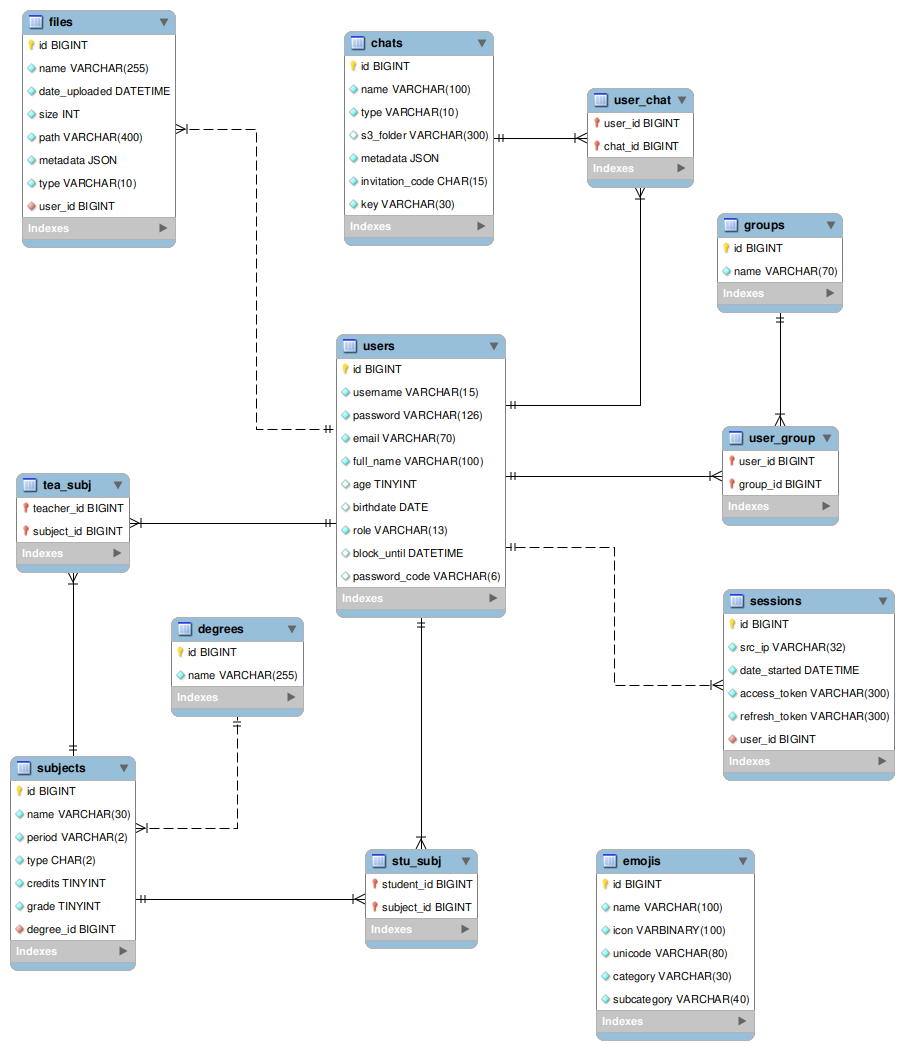
\includegraphics[width=0.8\textwidth]{diagramaBD}
	\caption{Diagrama de las tablas de la base de datos}
	\label{fig:diagrama-tablas}
\end{figure}

\sect{Seguridad}{seguridad}

Para la prevención de ciberataques al servidor por parte de usuarios malintencionados, se han
establecido las medidas de seguridad que se detallan a continuación:

\begin{itemize}
	\item \textbf{Cifrado de la comunicación entre el servidor y los clientes}: Para evitar que los datos de los
	usuarios puedan ser interceptados por terceros, se ha establecido un cifrado de las comunicaciones.\ Para ello, se
	ha empleado el protocolo TLS, que permite cifrar la comunicación utilizando el certificado SSL que proporciona
	Let's Encrypt.\ Este certificado se ha generado automáticamente mediante su servicio gratuito de certificados y,
	utilizando la aplicación \texttt{Certbot}, se renueva automáticamente cada 90 días.\ El certificado se
	almacena en el servidor en el directorio \texttt{/etc/letsencrypt/live/}.

	\item \textbf{Configuración del servidor ssh}: Para evitar que los usuarios puedan acceder al servidor mediante
	ssh, se ha configurado para que únicamente se pueda acceder mediante claves ssh (no permitiendo usuario y
	contraseña).\ Estas claves se obtienen mediante el comando \texttt{ssh-keygen}, que genera un par de claves
	(pública y privada), y se ha copiado la clave pública del cliente en el fichero
	\texttt{/home/user/.ssh/authorized\_keys} del servidor.\ De esta forma, únicamente se puede acceder al servidor
	mediante la
	clave privada del cliente.

	\item \textbf{Configuración del servidor web}: Se ha limitado la redirección de puertos desde el router hasta el
	servidor web, de forma que únicamente se puede acceder a los siguientes puertos:

	\begin{itemize}
		\item \boldFont{22}: puerto de ssh.
		\item \boldFont{80}: puerto de http.
		\item \boldFont{4040}: puerto de la aplicación en entorno de producción.
		\item \boldFont{4041}: puerto de la base de datos de la aplicación.
		\item \boldFont{4042}: puerto del servicio NSFW\@.
		\item \boldFont{4046}: puerto del panel de administración de Grafana.
	\end{itemize}

	Además, se ha configurado el servidor web para que únicamente se pueda acceder mediante el protocolo
	https, y no mediante http, haciendo que los usuarios sean redirigidos automáticamente a https.

	\item \textbf{Configuración de la base de datos}: La base de datos solo es accesible desde el propio servidor web,
	por lo que el acceso está restringido a la red interna.\ Para poder conectarse a la base de datos desde el
	exterior, se debe utilizar la clave ssh del servidor web, de forma que se accede a este y, desde ahí, se
	puede acceder a la base de datos.
\end{itemize}

\sect{Pruebas}{pruebas}



		\input{chapters/resultados}
		\chaptr{Conclusiones}{conclusiones}

En este capítulo se incluyen las conclusiones obtenidas tras el desarrollo del proyecto, así como una valoración
personal sobre el resultado final, las futuras ampliaciones y problemas encontrados.

Los \boldFont{objetivos} que se han propuesto en la sección~\ref{sec:objectives} \boldFont{se han cumplido} en su
totalidad dentro del plazo estimado.\ Se ha
conseguido desarrollar la aplicación web propuesta, permitiendo a los usuarios interactuar en tiempo real mediante
mensajes de todo tipo, incluyendo el filtrado de imágenes inapropiadas.

Algunas de las \boldFont{ampliaciones} que se han considerado implementar en un futuro son las siguientes:

\begin{itemize}
	\item \boldFont{Más tipos de mensajes}: se podrían añadir más tipos de mensajes, como por ejemplo, mensajes de
	ubicación, mensajes de voz, etc.
	\item \boldFont{Filtros para otro tipo de mensajes}: integrar los filtros existentes para mensajes de vídeo, audio
	u otros.
	\item \boldFont{Reenvío de mensajes a otros grupos}: permitir a los usuarios reenviar mensajes a otros grupos.
\end{itemize}

En cuanto a los \boldFont{problemas} encontrados, el más significativo ha sido el despliegue de la aplicación en
producción.\ Al inicio del proyecto, se desplegó en dos clusters con el plan gratuito de Heroku (uno
para el frontend y otro para el backend), pero se tuvo que retirar la aplicación de esta plataforma
debido a que este servicio no es gratuito desde el 28 de noviembre de 2022.
Actualmente, el frontend está desplegado en Vercel y en cuanto al backend, se consideraron varias opciones:

\begin{itemize}
	\item Despliegue en \textit{Platform.sh}: plataforma de despliegue de aplicaciones en la nube.
	\item Despliegue en un servidor propio.
\end{itemize}

La primera opción no ha sido posible, ya que, tras una reunión con el encargado de \textit{Cloud Services} de la
plataforma, no se ha podido conseguir una cuenta gratuita para el despliegue de la aplicación durante su desarrollo.
Por lo tanto, se ha optado por la segunda opción, comprando un pequeño ordenador personal y desplegando el backend en
él.\ De esta manera, también se abarca el campo de la administración de sistemas y redes, ya que se ha tenido que
configurar el servidor para que la aplicación funcione correctamente y se pueda acceder a ella desde cualquier lugar
con conexión a Internet.

		\chaptr{Anexos}{anexos}

% ----------------------------------------------------------------------------------------------- %

\sect{Anexo A: Pila del producto}{anexoA}

Durante el desarrollo del proyecto se han realizado una serie de tareas, para las cuales se ha utilizado la
herramienta \boldFont{Notion}.
Esta herramienta proporciona una interfaz muy sencilla para la creación de tareas, con la
posibilidad de añadir etiquetas, asignar responsables, añadir comentarios a cada una de ellas,
entre otras funcionalidades.
A continuación, se incluye el fichero pdf generado por Notion con la pila del producto completa.\ Además, se puede
consultar la pila del producto de una manera más interactiva en el siguiente enlace:
\href{https://scastd00.notion.site/9c59c2812d8b440faa453924fef2f320?v=20f7c2f47dd64574ac57713e8efe2718}
{https://scastd00.notion.site/9c59c2812d8b440faa453924fef2f3
20?v=20f7c2f47dd64574ac57713e8efe2718}

% Generar el pdf a 57% de tamaño para que quepa el ancho de página incluyendo las notas de Notion.
\label{anx:product-backlog-notion}
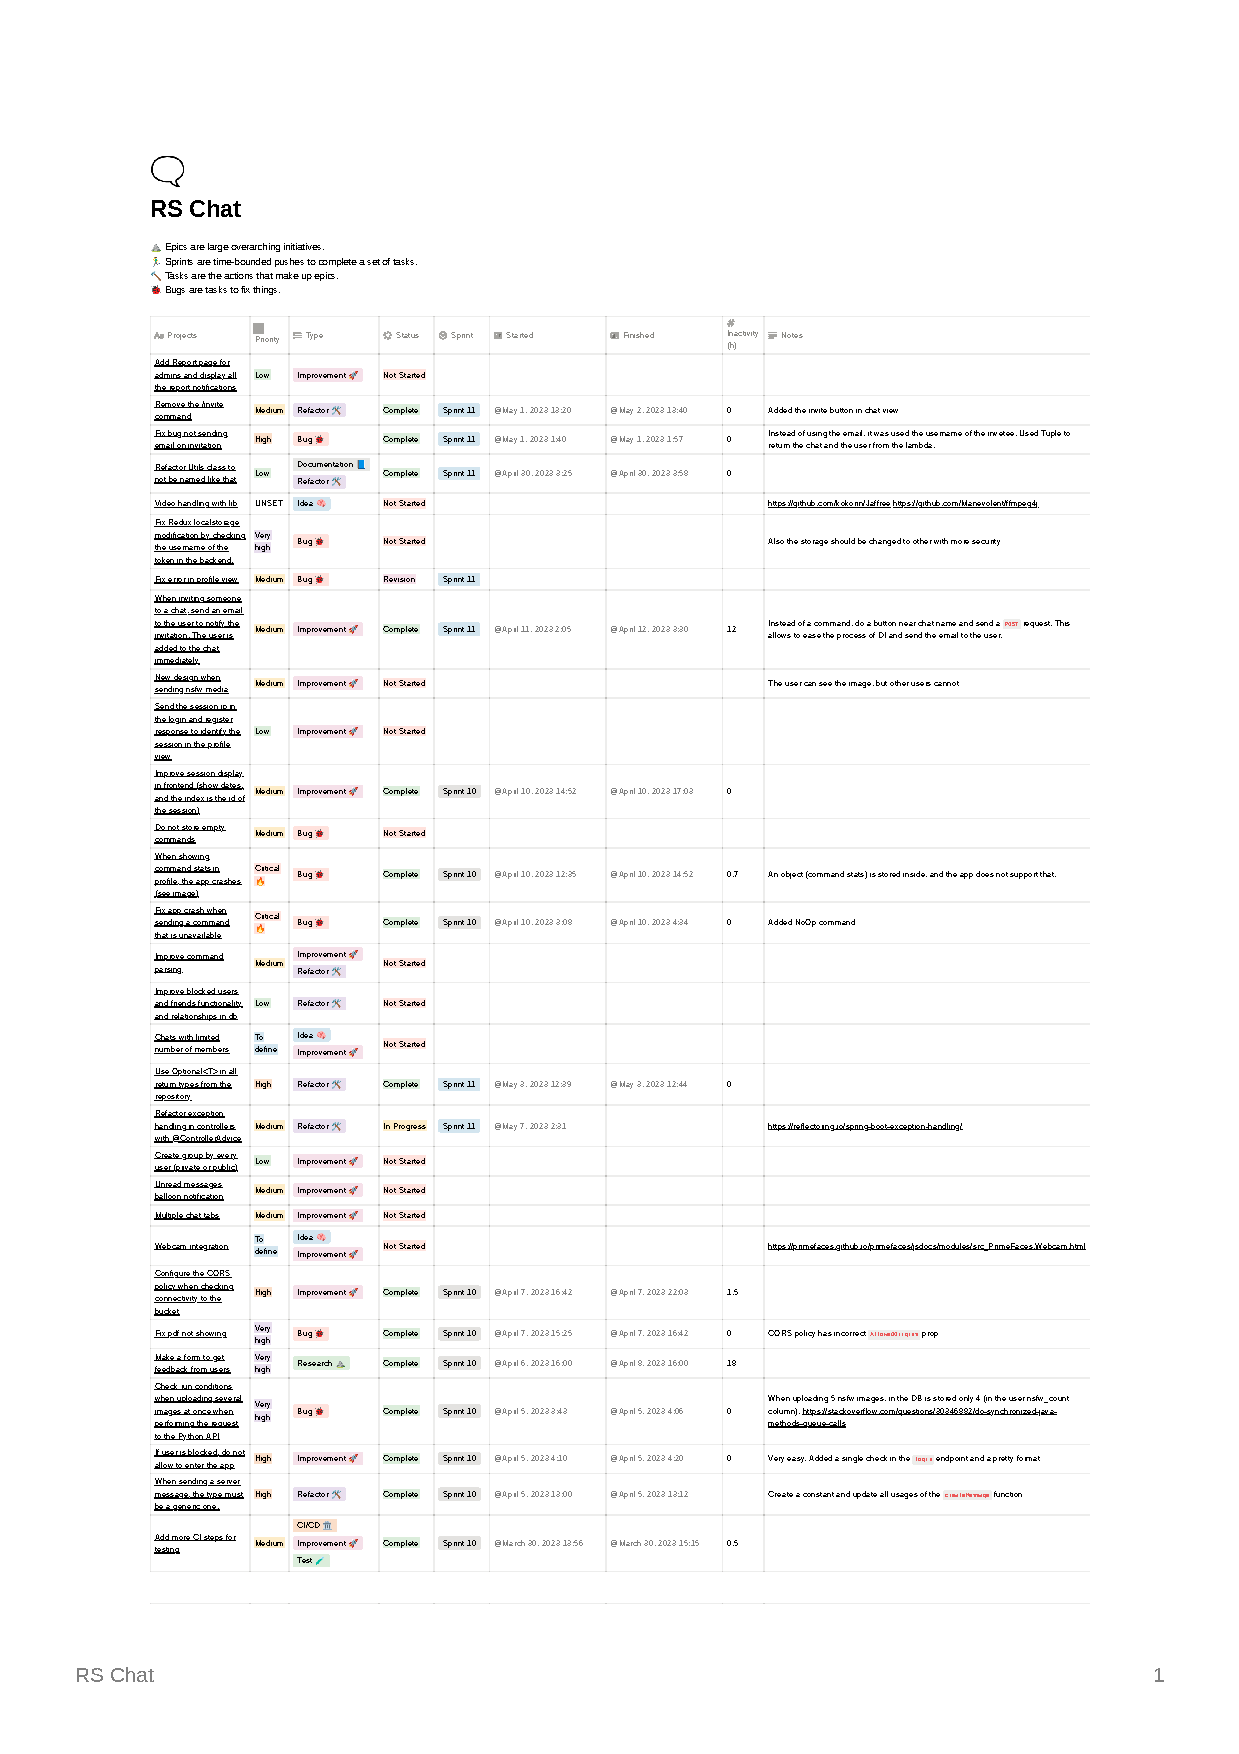
\includepdf[pages=-]{anexos/TareasNotion.pdf}

% ----------------------------------------------------------------------------------------------- %

\sect{Anexo B: Encuesta de satisfacción}{anexoB}

La encuesta de satisfacción realizada a los usuarios se puede visitar en el siguiente enlace:
\href{https://tally.so/r/31XyPQ}{https://tally.so/r/31XyPQ}
\label{anx:encuesta-satisfaccion}

% ----------------------------------------------------------------------------------------------- %

\sect{Anexo C: Diagramas de Gantt}{anexoC}

En esta sección se incluye el diagrama de Gantt completo del proyecto y el enlace a la hoja de cálculo de Google
Sheets con la que se ha generado.\ Además, esta contiene la pila del producto con las tareas completas y los diagramas
de Gantt de cada sprint de manera individual en hojas separadas.\ El enlace a la hoja de cálculo es el siguiente:
\href{https://docs.google.com/spreadsheets/d/1GOffJpsR0vORsQYvTrbWj72jmHIJvB0UMZqahqMcR-s/edit?usp=sharing}
{https://docs.google.com/spreadsheets/d/1GOffJpsR0vORsQYvTrbWj72jmHIJvB0U\\MZqahqMcR-s/edit?usp=sharing}

\label{anx:gantt}
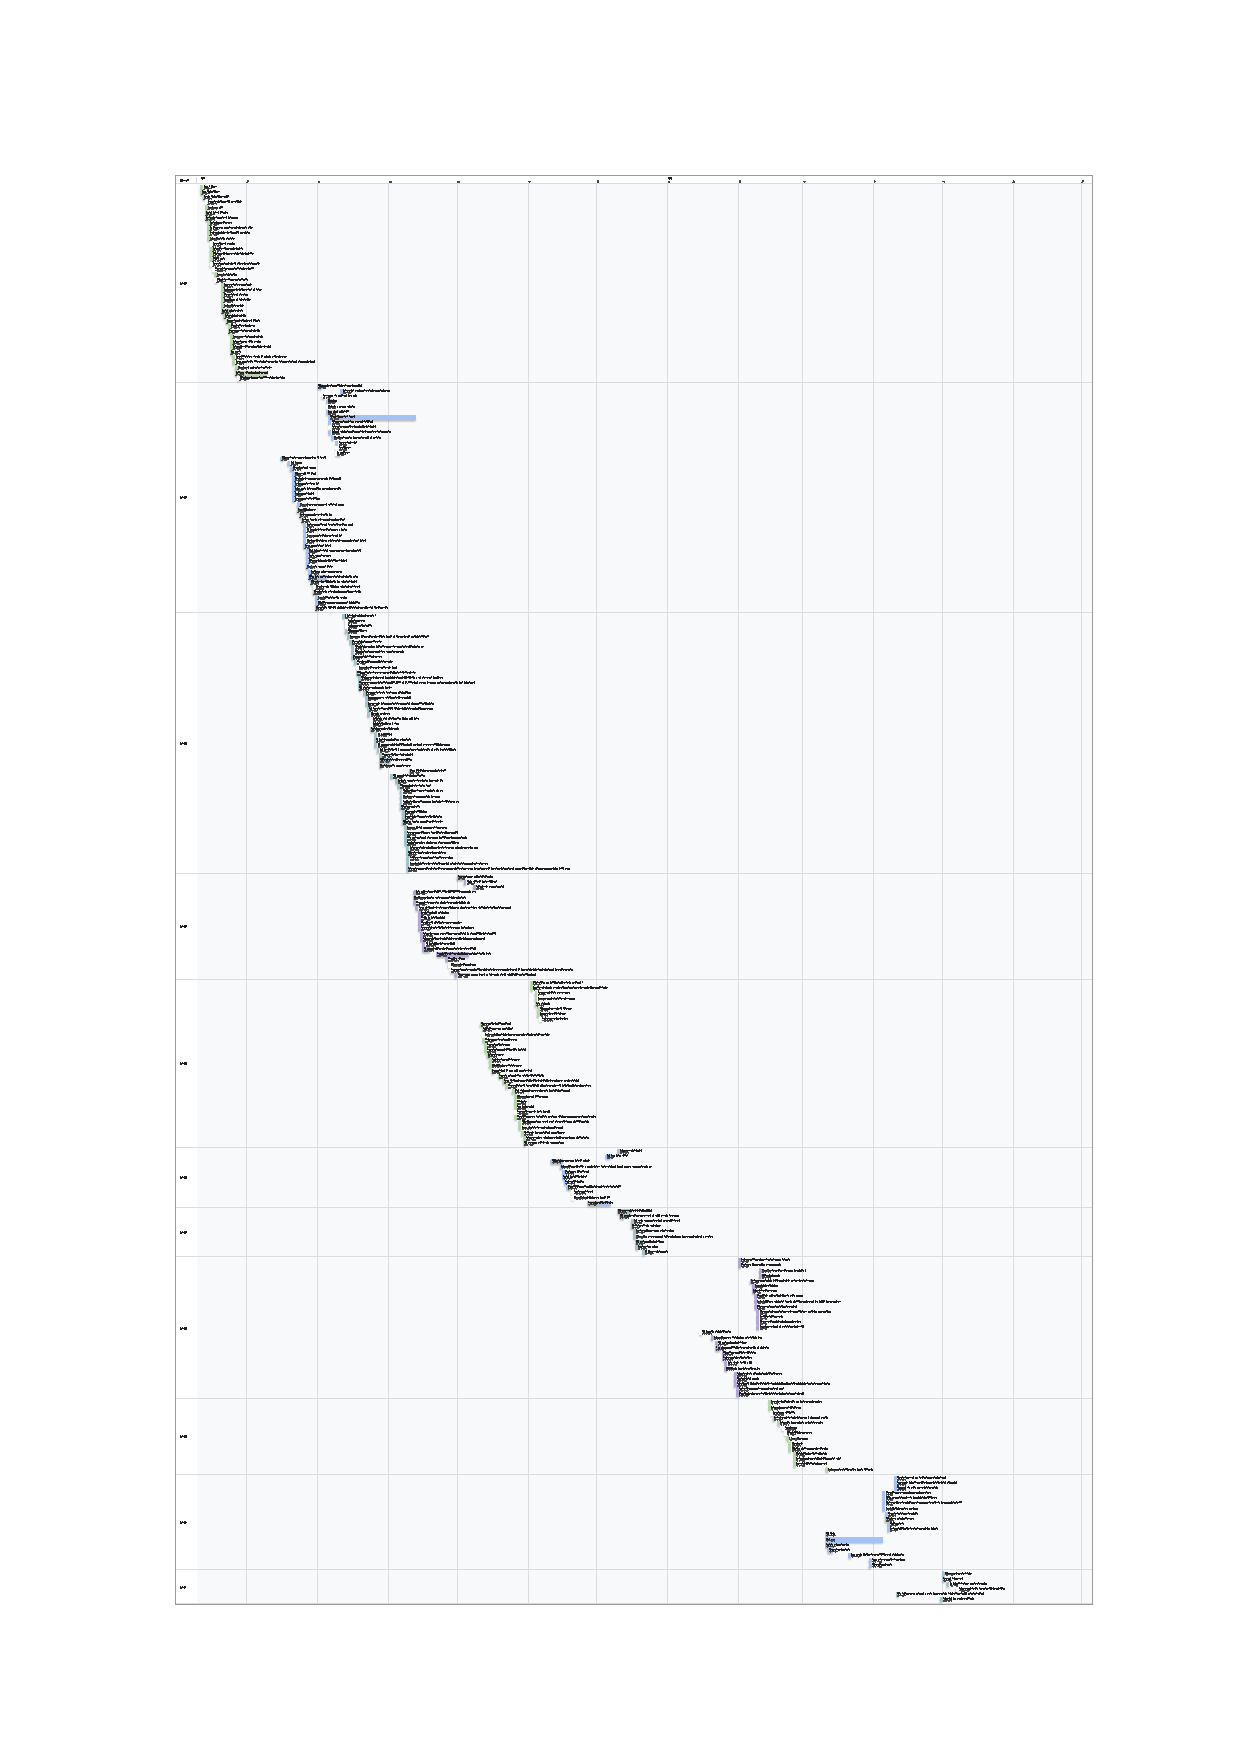
\includepdf[pages=-]{anexos/TodosLosSprints.pdf}

% ----------------------------------------------------------------------------------------------- %

\sect{Anexo D: Manual de usuario}{anexoD}

	\end{spacing}

	\cleardoublepage
	\addcontentsline{toc}{chapter}{Bibliografía}

	\printbibliography
\end{document}
